% Options for packages loaded elsewhere
\PassOptionsToPackage{unicode}{hyperref}
\PassOptionsToPackage{hyphens}{url}
%
\documentclass[
]{article}
\usepackage{amsmath,amssymb}
\usepackage{lmodern}
\usepackage{ifxetex,ifluatex}
\ifnum 0\ifxetex 1\fi\ifluatex 1\fi=0 % if pdftex
  \usepackage[T1]{fontenc}
  \usepackage[utf8]{inputenc}
  \usepackage{textcomp} % provide euro and other symbols
\else % if luatex or xetex
  \usepackage{unicode-math}
  \defaultfontfeatures{Scale=MatchLowercase}
  \defaultfontfeatures[\rmfamily]{Ligatures=TeX,Scale=1}
\fi
% Use upquote if available, for straight quotes in verbatim environments
\IfFileExists{upquote.sty}{\usepackage{upquote}}{}
\IfFileExists{microtype.sty}{% use microtype if available
  \usepackage[]{microtype}
  \UseMicrotypeSet[protrusion]{basicmath} % disable protrusion for tt fonts
}{}
\makeatletter
\@ifundefined{KOMAClassName}{% if non-KOMA class
  \IfFileExists{parskip.sty}{%
    \usepackage{parskip}
  }{% else
    \setlength{\parindent}{0pt}
    \setlength{\parskip}{6pt plus 2pt minus 1pt}}
}{% if KOMA class
  \KOMAoptions{parskip=half}}
\makeatother
\usepackage{xcolor}
\IfFileExists{xurl.sty}{\usepackage{xurl}}{} % add URL line breaks if available
\IfFileExists{bookmark.sty}{\usepackage{bookmark}}{\usepackage{hyperref}}
\hypersetup{
  pdftitle={Survival Analysis, Algorithmic Fairness, and COMPAS Recidivism Algorithm Case Study},
  pdfauthor={Octavio Mesner},
  hidelinks,
  pdfcreator={LaTeX via pandoc}}
\urlstyle{same} % disable monospaced font for URLs
\usepackage[margin=1in]{geometry}
\usepackage{color}
\usepackage{fancyvrb}
\newcommand{\VerbBar}{|}
\newcommand{\VERB}{\Verb[commandchars=\\\{\}]}
\DefineVerbatimEnvironment{Highlighting}{Verbatim}{commandchars=\\\{\}}
% Add ',fontsize=\small' for more characters per line
\usepackage{framed}
\definecolor{shadecolor}{RGB}{248,248,248}
\newenvironment{Shaded}{\begin{snugshade}}{\end{snugshade}}
\newcommand{\AlertTok}[1]{\textcolor[rgb]{0.94,0.16,0.16}{#1}}
\newcommand{\AnnotationTok}[1]{\textcolor[rgb]{0.56,0.35,0.01}{\textbf{\textit{#1}}}}
\newcommand{\AttributeTok}[1]{\textcolor[rgb]{0.77,0.63,0.00}{#1}}
\newcommand{\BaseNTok}[1]{\textcolor[rgb]{0.00,0.00,0.81}{#1}}
\newcommand{\BuiltInTok}[1]{#1}
\newcommand{\CharTok}[1]{\textcolor[rgb]{0.31,0.60,0.02}{#1}}
\newcommand{\CommentTok}[1]{\textcolor[rgb]{0.56,0.35,0.01}{\textit{#1}}}
\newcommand{\CommentVarTok}[1]{\textcolor[rgb]{0.56,0.35,0.01}{\textbf{\textit{#1}}}}
\newcommand{\ConstantTok}[1]{\textcolor[rgb]{0.00,0.00,0.00}{#1}}
\newcommand{\ControlFlowTok}[1]{\textcolor[rgb]{0.13,0.29,0.53}{\textbf{#1}}}
\newcommand{\DataTypeTok}[1]{\textcolor[rgb]{0.13,0.29,0.53}{#1}}
\newcommand{\DecValTok}[1]{\textcolor[rgb]{0.00,0.00,0.81}{#1}}
\newcommand{\DocumentationTok}[1]{\textcolor[rgb]{0.56,0.35,0.01}{\textbf{\textit{#1}}}}
\newcommand{\ErrorTok}[1]{\textcolor[rgb]{0.64,0.00,0.00}{\textbf{#1}}}
\newcommand{\ExtensionTok}[1]{#1}
\newcommand{\FloatTok}[1]{\textcolor[rgb]{0.00,0.00,0.81}{#1}}
\newcommand{\FunctionTok}[1]{\textcolor[rgb]{0.00,0.00,0.00}{#1}}
\newcommand{\ImportTok}[1]{#1}
\newcommand{\InformationTok}[1]{\textcolor[rgb]{0.56,0.35,0.01}{\textbf{\textit{#1}}}}
\newcommand{\KeywordTok}[1]{\textcolor[rgb]{0.13,0.29,0.53}{\textbf{#1}}}
\newcommand{\NormalTok}[1]{#1}
\newcommand{\OperatorTok}[1]{\textcolor[rgb]{0.81,0.36,0.00}{\textbf{#1}}}
\newcommand{\OtherTok}[1]{\textcolor[rgb]{0.56,0.35,0.01}{#1}}
\newcommand{\PreprocessorTok}[1]{\textcolor[rgb]{0.56,0.35,0.01}{\textit{#1}}}
\newcommand{\RegionMarkerTok}[1]{#1}
\newcommand{\SpecialCharTok}[1]{\textcolor[rgb]{0.00,0.00,0.00}{#1}}
\newcommand{\SpecialStringTok}[1]{\textcolor[rgb]{0.31,0.60,0.02}{#1}}
\newcommand{\StringTok}[1]{\textcolor[rgb]{0.31,0.60,0.02}{#1}}
\newcommand{\VariableTok}[1]{\textcolor[rgb]{0.00,0.00,0.00}{#1}}
\newcommand{\VerbatimStringTok}[1]{\textcolor[rgb]{0.31,0.60,0.02}{#1}}
\newcommand{\WarningTok}[1]{\textcolor[rgb]{0.56,0.35,0.01}{\textbf{\textit{#1}}}}
\usepackage{longtable,booktabs,array}
\usepackage{calc} % for calculating minipage widths
% Correct order of tables after \paragraph or \subparagraph
\usepackage{etoolbox}
\makeatletter
\patchcmd\longtable{\par}{\if@noskipsec\mbox{}\fi\par}{}{}
\makeatother
% Allow footnotes in longtable head/foot
\IfFileExists{footnotehyper.sty}{\usepackage{footnotehyper}}{\usepackage{footnote}}
\makesavenoteenv{longtable}
\usepackage{graphicx}
\makeatletter
\def\maxwidth{\ifdim\Gin@nat@width>\linewidth\linewidth\else\Gin@nat@width\fi}
\def\maxheight{\ifdim\Gin@nat@height>\textheight\textheight\else\Gin@nat@height\fi}
\makeatother
% Scale images if necessary, so that they will not overflow the page
% margins by default, and it is still possible to overwrite the defaults
% using explicit options in \includegraphics[width, height, ...]{}
\setkeys{Gin}{width=\maxwidth,height=\maxheight,keepaspectratio}
% Set default figure placement to htbp
\makeatletter
\def\fps@figure{htbp}
\makeatother
\setlength{\emergencystretch}{3em} % prevent overfull lines
\providecommand{\tightlist}{%
  \setlength{\itemsep}{0pt}\setlength{\parskip}{0pt}}
\setcounter{secnumdepth}{-\maxdimen} % remove section numbering
\usepackage{tikz}
\usepackage{pgfplots}
\ifluatex
  \usepackage{selnolig}  % disable illegal ligatures
\fi

\title{Survival Analysis, Algorithmic Fairness, and COMPAS Recidivism
Algorithm Case Study}
\author{Octavio Mesner}
\date{}

\begin{document}
\maketitle

\hypertarget{consulting-skills-focus}{%
\subsection{Consulting Skills Focus}\label{consulting-skills-focus}}

\begin{itemize}
\item
  In real life consulting, the client will frequently understand the
  data and surrounding research better than the data
  scientist/statistician.
\item
  Analysis should center around a well-defined research question that
  drive the analysis and the data should be able to provide insight on
  the question of interest.
\item
  Human bias and data analysis: We all have bias. This can influence
  data analysis. A data analyst, we should do our best to objectively
  present the data. When necessary to make assumptions, state them
  explicitly.\\
\item
  Publication Bias example: Researchers frequently want ``positive
  results.'' Usually this means significant p-values. Variable selection
  is a simple way to change p-values, p-hacking. It's common to need to
  change variables in a model be it should be done a principled way.
\item
  Question: Have you heard of field of
  \href{https://en.wikipedia.org/wiki/Fairness_(machine_learning)}{algorithmic
  fairness}?

  \begin{itemize}
  \item
    \begin{enumerate}
    \def\labelenumi{\alph{enumi})}
    \tightlist
    \item
      yes
    \end{enumerate}
  \item
    \begin{enumerate}
    \def\labelenumi{\alph{enumi})}
    \setcounter{enumi}{1}
    \tightlist
    \item
      no
    \end{enumerate}
  \end{itemize}
\end{itemize}

\hypertarget{case-study-background}{%
\subsection{Case Study Background}\label{case-study-background}}

\begin{itemize}
\item
  US has more inmates, proportional to population size, than any other
  country. While Black Americans make up 13\% of the total US
  population, they account for 40\% of incarcerated population in the
  US. 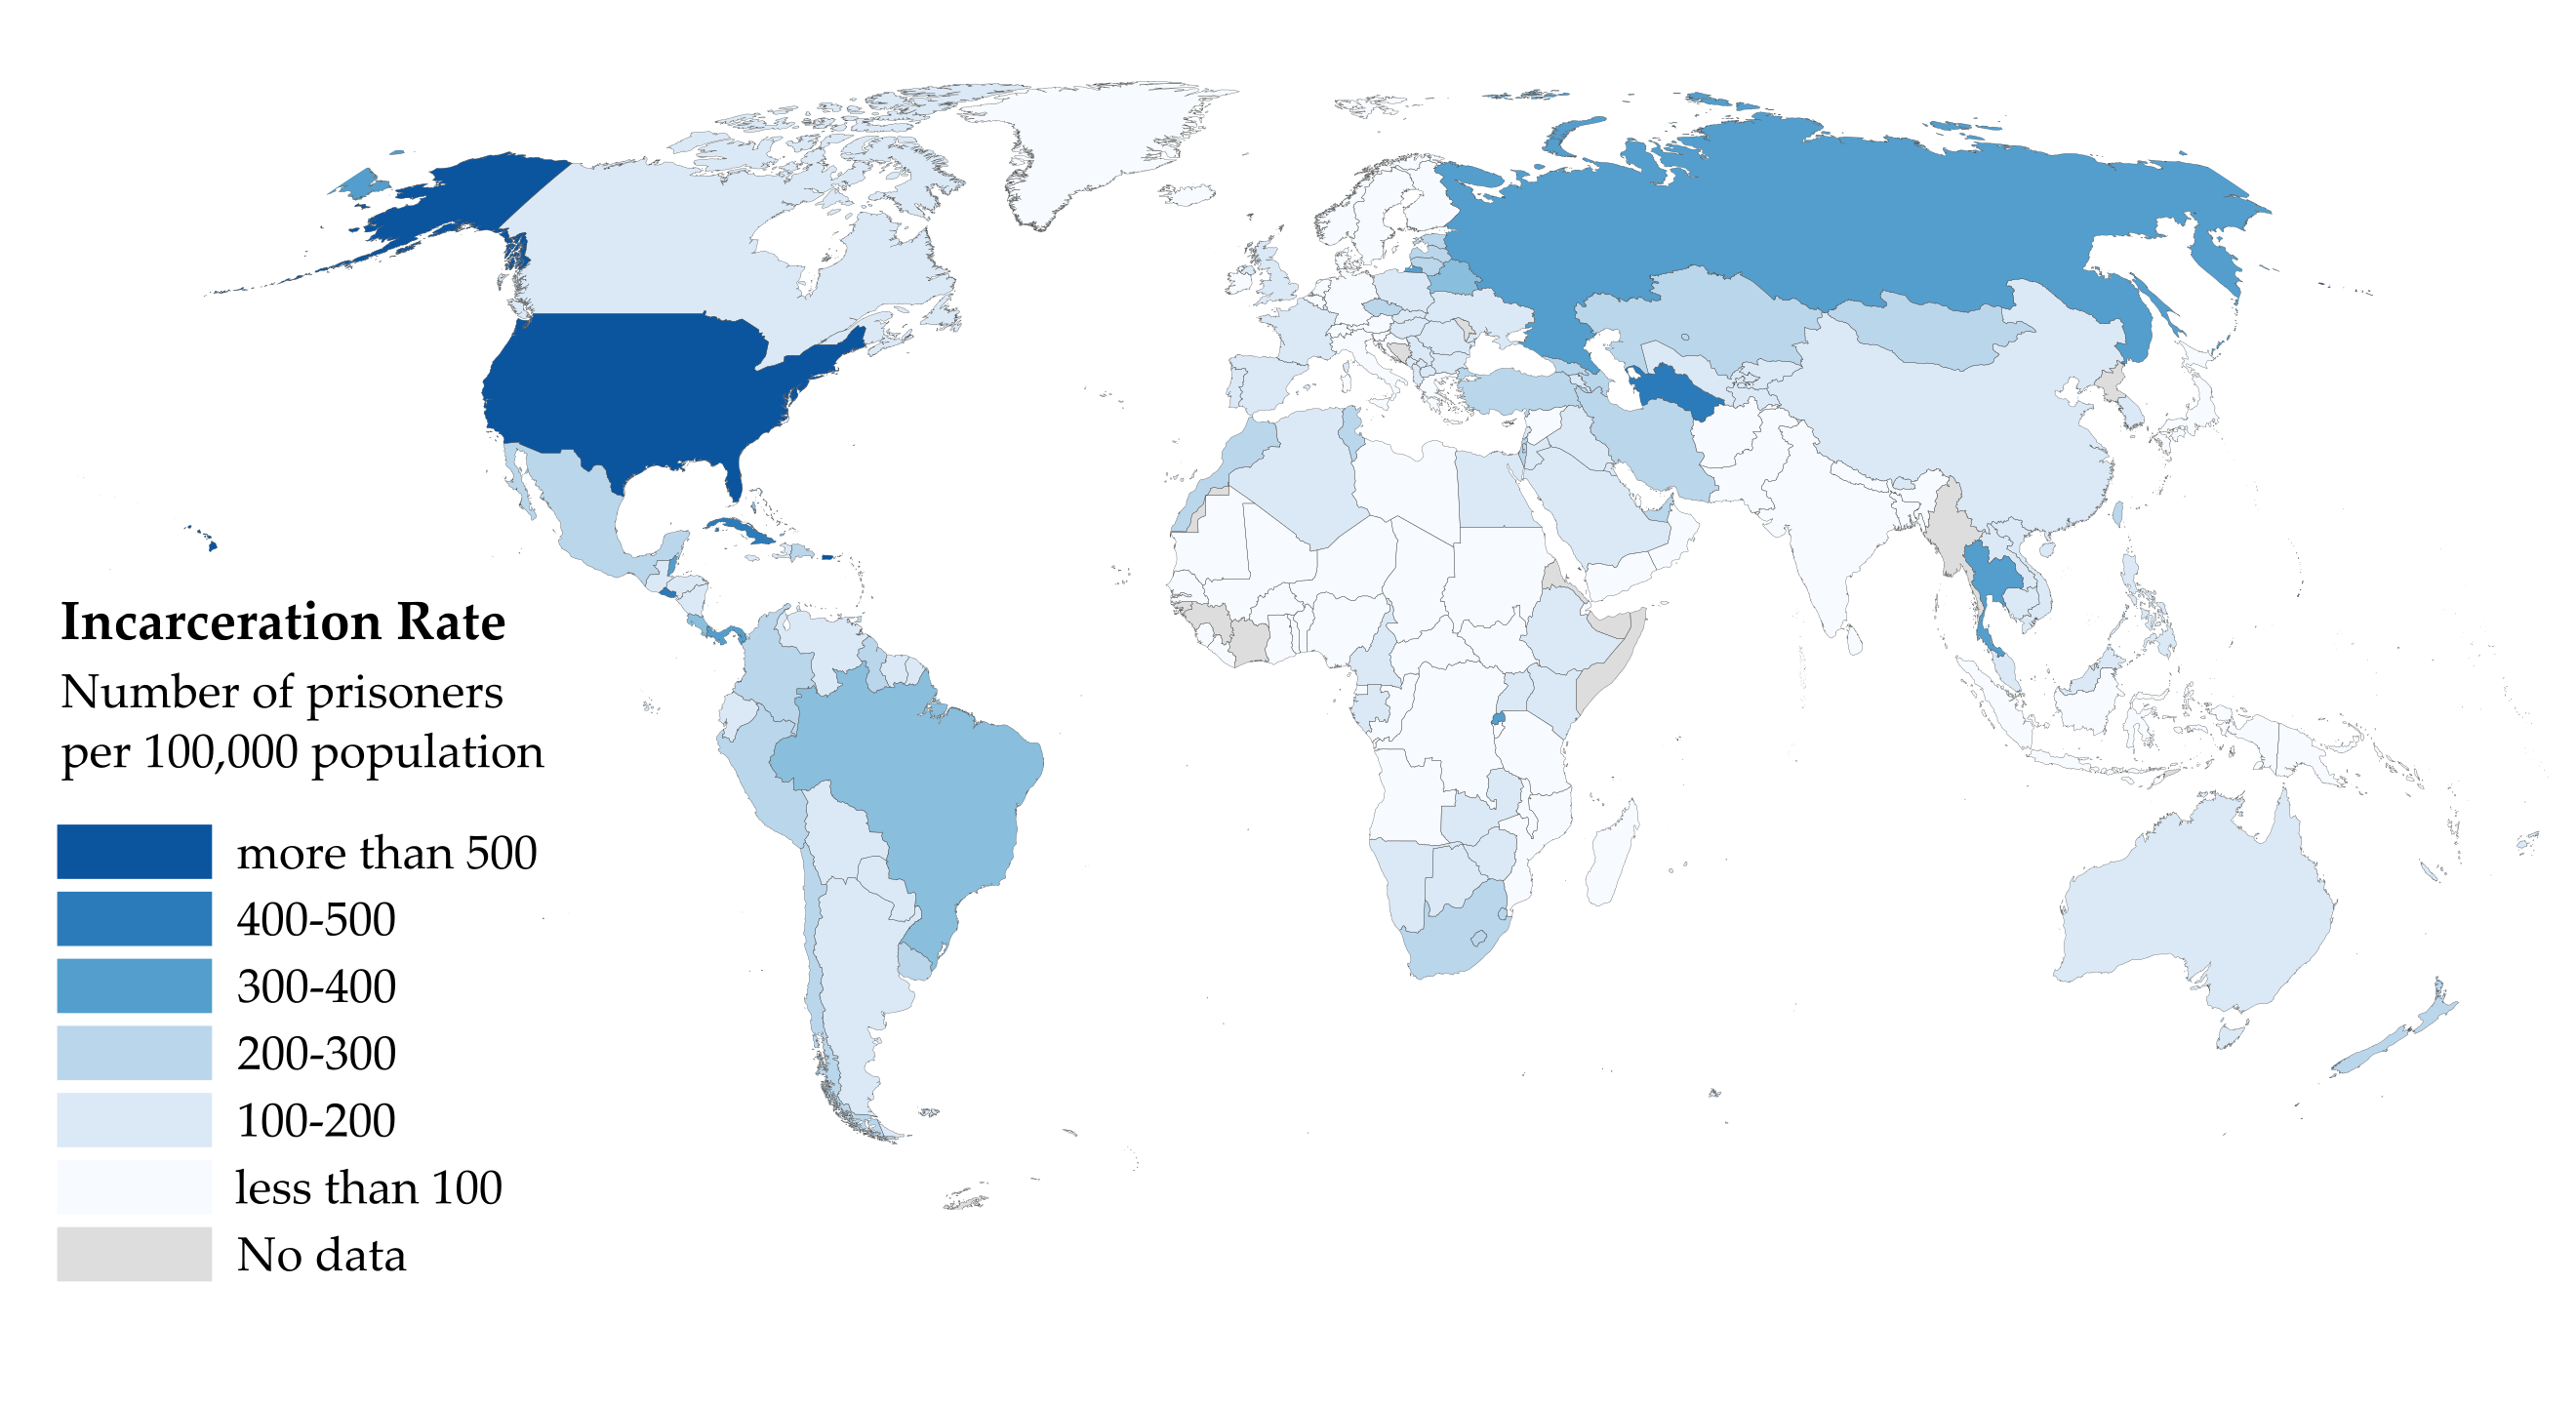
\includegraphics{./Prisoners_world_map_png2.png} Image from
  \href{https://en.wikipedia.org/wiki/Incarceration_in_the_United_States\#/media/File:Prisoners_world_map_png2.png}{Wikipedia}
\item
  In the US justice system, machine learning algorithms are sometimes
  used to assess a criminal defendant's risk of recidivism (arrest due
  to committing a future crime) are being used.
\item
  Correctional Offenders Management Profiling for Alternative Sanctions
  (COMPAS) is the most widespread of these algorithms.
\item
  Its goal according to COMPAS creators: assess ``not just risk but also
  nearly two dozen so-called ``criminogenic needs'' that relate to the
  major theories of criminality, including ``criminal personality,''
  ``social isolation,'' ``substance abuse'' and ``residence/stability.''
  Defendants are ranked low, medium or high risk in each category."
\item
  In 2014, then U.S. Attorney General Eric Holder warned that the risk
  scores might be injecting bias into the courts. He called for the U.S.
  Sentencing Commission to study their use. ``Although these measures
  were crafted with the best of intentions, I am concerned that they
  inadvertently undermine our efforts to ensure individualized and equal
  justice,'' he said, adding, ``they may exacerbate unwarranted and
  unjust disparities that are already far too common in our criminal
  justice system and in our society.''
\item
  The
  \href{https://www.documentcloud.org/documents/2702103-Sample-Risk-Assessment-COMPAS-CORE.html}{questionnaire}
  for determining COMPAS does not directly ask for race, but some people
  question inherent racial bias in the algorithm.
\item
  The COMPAS algorithm is proprietary and not available.
\item
  More information in a
  \href{https://www.propublica.org/article/machine-bias-risk-assessments-in-criminal-sentencing}{2016
  ProPublica article}.
\end{itemize}

\hypertarget{data}{%
\subsection{Data}\label{data}}

\begin{itemize}
\item
  ProPublica requested two years of COMPAS scores from Broward County
  Sheriff's Office in Florida
\item
  Discarded all but pre-trial COMPAS score assessments
\item
  ProPublica matched COMPAS scores with criminal records from Broward
  County Clerk's Office website
\item
  COMPAS score screening date and (original) arrest date frequently
  differed. If they are too far apart, that may indicate an error. The
  \texttt{days\_b\_screening\_arrest} variable gives this difference in
  days.
\item
  \texttt{is\_recid} is rearrest at any time. \texttt{two\_year\_recid}
  is rearrest within two years. Here, \texttt{-1} indicates a COMPAS
  record could not be found and should probably be discarded
\item
  COMPAS generates a general score, \texttt{decile\_score}, (1,
  2,\ldots,10) where 1 indicates a low risk and 10 indicates a high risk
  of recidivism. There is also a violence score as well,
  \texttt{v\_decile\_score}.
\end{itemize}

\begin{Shaded}
\begin{Highlighting}[]
\NormalTok{dat}\OtherTok{\textless{}{-}}\FunctionTok{read.csv}\NormalTok{(}\StringTok{"./compas{-}scores.csv"}\NormalTok{)}
\FunctionTok{dim}\NormalTok{(dat)}
\end{Highlighting}
\end{Shaded}

\begin{verbatim}
## [1] 11757    47
\end{verbatim}

\begin{Shaded}
\begin{Highlighting}[]
\FunctionTok{names}\NormalTok{(dat)}
\end{Highlighting}
\end{Shaded}

\begin{verbatim}
##  [1] "id"                      "name"                   
##  [3] "first"                   "last"                   
##  [5] "compas_screening_date"   "sex"                    
##  [7] "dob"                     "age"                    
##  [9] "age_cat"                 "race"                   
## [11] "juv_fel_count"           "decile_score"           
## [13] "juv_misd_count"          "juv_other_count"        
## [15] "priors_count"            "days_b_screening_arrest"
## [17] "c_jail_in"               "c_jail_out"             
## [19] "c_case_number"           "c_offense_date"         
## [21] "c_arrest_date"           "c_days_from_compas"     
## [23] "c_charge_degree"         "c_charge_desc"          
## [25] "is_recid"                "num_r_cases"            
## [27] "r_case_number"           "r_charge_degree"        
## [29] "r_days_from_arrest"      "r_offense_date"         
## [31] "r_charge_desc"           "r_jail_in"              
## [33] "r_jail_out"              "is_violent_recid"       
## [35] "num_vr_cases"            "vr_case_number"         
## [37] "vr_charge_degree"        "vr_offense_date"        
## [39] "vr_charge_desc"          "v_type_of_assessment"   
## [41] "v_decile_score"          "v_score_text"           
## [43] "v_screening_date"        "type_of_assessment"     
## [45] "decile_score.1"          "score_text"             
## [47] "screening_date"
\end{verbatim}

\begin{Shaded}
\begin{Highlighting}[]
\FunctionTok{head}\NormalTok{(dat[,}\DecValTok{1}\SpecialCharTok{:}\DecValTok{12}\NormalTok{])}
\end{Highlighting}
\end{Shaded}

\begin{verbatim}
##   id               name   first        last compas_screening_date  sex
## 1  1   miguel hernandez  miguel   hernandez            2013-08-14 Male
## 2  2       michael ryan michael        ryan            2014-12-31 Male
## 3  3        kevon dixon   kevon       dixon            2013-01-27 Male
## 4  4           ed philo      ed       philo            2013-04-14 Male
## 5  5        marcu brown   marcu       brown            2013-01-13 Male
## 6  6 bouthy pierrelouis  bouthy pierrelouis            2013-03-26 Male
##          dob age         age_cat             race juv_fel_count decile_score
## 1 1947-04-18  69 Greater than 45            Other             0            1
## 2 1985-02-06  31         25 - 45        Caucasian             0            5
## 3 1982-01-22  34         25 - 45 African-American             0            3
## 4 1991-05-14  24    Less than 25 African-American             0            4
## 5 1993-01-21  23    Less than 25 African-American             0            8
## 6 1973-01-22  43         25 - 45            Other             0            1
\end{verbatim}

\begin{Shaded}
\begin{Highlighting}[]
\FunctionTok{summary}\NormalTok{(dat)}
\end{Highlighting}
\end{Shaded}

\begin{verbatim}
##        id            name              first               last          
##  Min.   :    1   Length:11757       Length:11757       Length:11757      
##  1st Qu.: 2940   Class :character   Class :character   Class :character  
##  Median : 5879   Mode  :character   Mode  :character   Mode  :character  
##  Mean   : 5879                                                           
##  3rd Qu.: 8818                                                           
##  Max.   :11757                                                           
##                                                                          
##  compas_screening_date     sex                dob                 age       
##  Length:11757          Length:11757       Length:11757       Min.   :18.00  
##  Class :character      Class :character   Class :character   1st Qu.:25.00  
##  Mode  :character      Mode  :character   Mode  :character   Median :32.00  
##                                                              Mean   :35.14  
##                                                              3rd Qu.:43.00  
##                                                              Max.   :96.00  
##                                                                             
##    age_cat              race           juv_fel_count       decile_score   
##  Length:11757       Length:11757       Min.   : 0.00000   Min.   :-1.000  
##  Class :character   Class :character   1st Qu.: 0.00000   1st Qu.: 2.000  
##  Mode  :character   Mode  :character   Median : 0.00000   Median : 4.000  
##                                        Mean   : 0.06158   Mean   : 4.371  
##                                        3rd Qu.: 0.00000   3rd Qu.: 7.000  
##                                        Max.   :20.00000   Max.   :10.000  
##                                                                           
##  juv_misd_count     juv_other_count     priors_count    days_b_screening_arrest
##  Min.   : 0.00000   Min.   : 0.00000   Min.   : 0.000   Min.   :-597.000       
##  1st Qu.: 0.00000   1st Qu.: 0.00000   1st Qu.: 0.000   1st Qu.:  -1.000       
##  Median : 0.00000   Median : 0.00000   Median : 1.000   Median :  -1.000       
##  Mean   : 0.07604   Mean   : 0.09356   Mean   : 3.082   Mean   :  -0.878       
##  3rd Qu.: 0.00000   3rd Qu.: 0.00000   3rd Qu.: 4.000   3rd Qu.:  -1.000       
##  Max.   :13.00000   Max.   :17.00000   Max.   :43.000   Max.   :1057.000       
##                                                         NA's   :1180           
##   c_jail_in          c_jail_out        c_case_number      c_offense_date    
##  Length:11757       Length:11757       Length:11757       Length:11757      
##  Class :character   Class :character   Class :character   Class :character  
##  Mode  :character   Mode  :character   Mode  :character   Mode  :character  
##                                                                             
##                                                                             
##                                                                             
##                                                                             
##  c_arrest_date      c_days_from_compas c_charge_degree    c_charge_desc     
##  Length:11757       Min.   :   0.00    Length:11757       Length:11757      
##  Class :character   1st Qu.:   1.00    Class :character   Class :character  
##  Mode  :character   Median :   1.00    Mode  :character   Mode  :character  
##                     Mean   :  63.59                                         
##                     3rd Qu.:   2.00                                         
##                     Max.   :9485.00                                         
##                     NA's   :742                                             
##     is_recid       num_r_cases    r_case_number      r_charge_degree   
##  Min.   :-1.0000   Mode:logical   Length:11757       Length:11757      
##  1st Qu.: 0.0000   NA's:11757     Class :character   Class :character  
##  Median : 0.0000                  Mode  :character   Mode  :character  
##  Mean   : 0.2538                                                       
##  3rd Qu.: 1.0000                                                       
##  Max.   : 1.0000                                                       
##                                                                        
##  r_days_from_arrest r_offense_date     r_charge_desc       r_jail_in        
##  Min.   : -1.00     Length:11757       Length:11757       Length:11757      
##  1st Qu.:  0.00     Class :character   Class :character   Class :character  
##  Median :  0.00     Mode  :character   Mode  :character   Mode  :character  
##  Mean   : 20.41                                                             
##  3rd Qu.:  1.00                                                             
##  Max.   :993.00                                                             
##  NA's   :9297                                                               
##   r_jail_out        is_violent_recid  num_vr_cases   vr_case_number    
##  Length:11757       Min.   :0.00000   Mode:logical   Length:11757      
##  Class :character   1st Qu.:0.00000   NA's:11757     Class :character  
##  Mode  :character   Median :0.00000                  Mode  :character  
##                     Mean   :0.07502                                    
##                     3rd Qu.:0.00000                                    
##                     Max.   :1.00000                                    
##                                                                        
##  vr_charge_degree   vr_offense_date    vr_charge_desc     v_type_of_assessment
##  Length:11757       Length:11757       Length:11757       Length:11757        
##  Class :character   Class :character   Class :character   Class :character    
##  Mode  :character   Mode  :character   Mode  :character   Mode  :character    
##                                                                               
##                                                                               
##                                                                               
##                                                                               
##  v_decile_score   v_score_text       v_screening_date   type_of_assessment
##  Min.   :-1.000   Length:11757       Length:11757       Length:11757      
##  1st Qu.: 1.000   Class :character   Class :character   Class :character  
##  Median : 3.000   Mode  :character   Mode  :character   Mode  :character  
##  Mean   : 3.571                                                           
##  3rd Qu.: 5.000                                                           
##  Max.   :10.000                                                           
##                                                                           
##  decile_score.1    score_text        screening_date    
##  Min.   :-1.000   Length:11757       Length:11757      
##  1st Qu.: 2.000   Class :character   Class :character  
##  Median : 4.000   Mode  :character   Mode  :character  
##  Mean   : 4.371                                        
##  3rd Qu.: 7.000                                        
##  Max.   :10.000                                        
## 
\end{verbatim}

Are there multiple rows per person?

\begin{Shaded}
\begin{Highlighting}[]
\FunctionTok{length}\NormalTok{(}\FunctionTok{unique}\NormalTok{(dat}\SpecialCharTok{$}\NormalTok{id))}
\end{Highlighting}
\end{Shaded}

\begin{verbatim}
## [1] 11757
\end{verbatim}

\begin{Shaded}
\begin{Highlighting}[]
\FunctionTok{length}\NormalTok{(dat}\SpecialCharTok{$}\NormalTok{id)}
\end{Highlighting}
\end{Shaded}

\begin{verbatim}
## [1] 11757
\end{verbatim}

\begin{Shaded}
\begin{Highlighting}[]
\FunctionTok{length}\NormalTok{(}\FunctionTok{unique}\NormalTok{(dat}\SpecialCharTok{$}\NormalTok{name))}
\end{Highlighting}
\end{Shaded}

\begin{verbatim}
## [1] 11584
\end{verbatim}

\begin{Shaded}
\begin{Highlighting}[]
\FunctionTok{sort}\NormalTok{(}\FunctionTok{table}\NormalTok{(dat}\SpecialCharTok{$}\NormalTok{name), }\AttributeTok{decreasing=}\ConstantTok{TRUE}\NormalTok{)[}\DecValTok{1}\SpecialCharTok{:}\DecValTok{8}\NormalTok{]}
\end{Highlighting}
\end{Shaded}

\begin{verbatim}
## 
##     carlos vasquez         john brown michael cunningham      robert taylor 
##                  4                  4                  4                  4 
##    anthony jackson      anthony smith   gregory williams        james brown 
##                  3                  3                  3                  3
\end{verbatim}

\begin{itemize}
\item
  To me, these seem like common names, so it could be a coincidence, but
  I would check with the client as due diligence
\item
  What else could we do to check?
\end{itemize}

What about other demographics?

\begin{Shaded}
\begin{Highlighting}[]
\FunctionTok{table}\NormalTok{(dat}\SpecialCharTok{$}\NormalTok{sex)}
\end{Highlighting}
\end{Shaded}

\begin{verbatim}
## 
## Female   Male 
##   2421   9336
\end{verbatim}

\begin{Shaded}
\begin{Highlighting}[]
\FunctionTok{table}\NormalTok{(dat}\SpecialCharTok{$}\NormalTok{sex)}\SpecialCharTok{/}\FunctionTok{sum}\NormalTok{(}\SpecialCharTok{!}\FunctionTok{is.na}\NormalTok{(dat}\SpecialCharTok{$}\NormalTok{sex))}\SpecialCharTok{*}\DecValTok{100}
\end{Highlighting}
\end{Shaded}

\begin{verbatim}
## 
##   Female     Male 
## 20.59199 79.40801
\end{verbatim}

\begin{Shaded}
\begin{Highlighting}[]
\FunctionTok{library}\NormalTok{(ggplot2)}
\FunctionTok{ggplot}\NormalTok{(dat, }\FunctionTok{aes}\NormalTok{(}\AttributeTok{x=}\NormalTok{age, }\AttributeTok{color=}\NormalTok{sex, }\AttributeTok{fill=}\NormalTok{sex)) }\SpecialCharTok{+}
  \FunctionTok{geom\_histogram}\NormalTok{(}\AttributeTok{position=}\StringTok{"dodge"}\NormalTok{)}
\end{Highlighting}
\end{Shaded}

\begin{verbatim}
## `stat_bin()` using `bins = 30`. Pick better value with `binwidth`.
\end{verbatim}

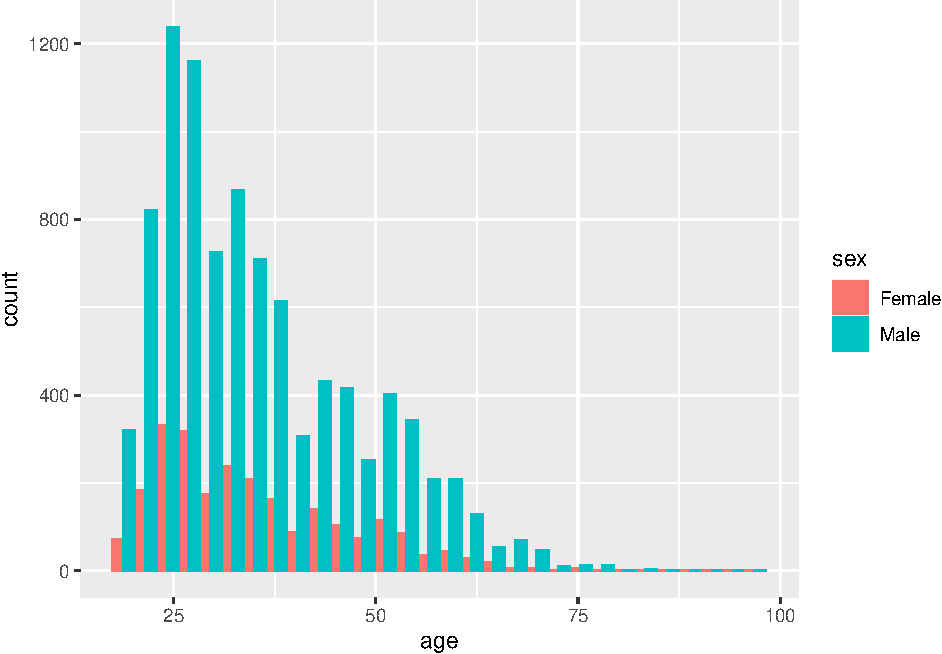
\includegraphics{survival_files/figure-latex/age-1.pdf}

\begin{Shaded}
\begin{Highlighting}[]
\FunctionTok{ggplot}\NormalTok{(dat, }\FunctionTok{aes}\NormalTok{(race)) }\SpecialCharTok{+}
  \FunctionTok{geom\_bar}\NormalTok{(}\AttributeTok{fill=}\StringTok{\textquotesingle{}blue\textquotesingle{}}\NormalTok{)}
\end{Highlighting}
\end{Shaded}

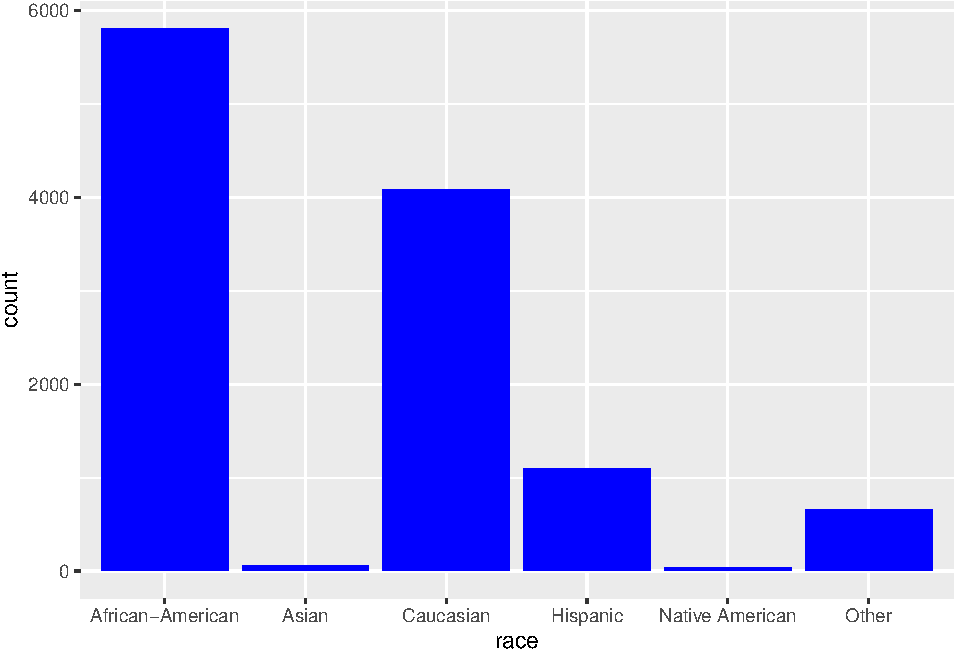
\includegraphics{survival_files/figure-latex/race-1.pdf}

\begin{Shaded}
\begin{Highlighting}[]
\FunctionTok{ggplot}\NormalTok{(dat, }\FunctionTok{aes}\NormalTok{(}\AttributeTok{x=}\NormalTok{race, }\AttributeTok{fill=}\NormalTok{sex)) }\SpecialCharTok{+}
  \FunctionTok{geom\_bar}\NormalTok{(}\AttributeTok{position=}\StringTok{\textquotesingle{}dodge\textquotesingle{}}\NormalTok{)}
\end{Highlighting}
\end{Shaded}

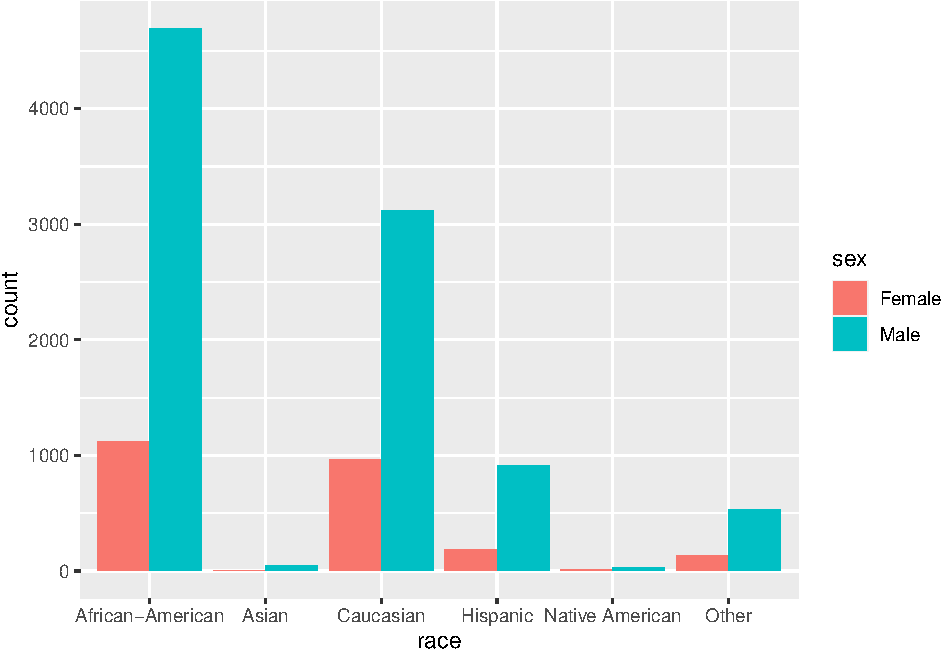
\includegraphics{survival_files/figure-latex/race-2.pdf}

\begin{Shaded}
\begin{Highlighting}[]
\FunctionTok{ggplot}\NormalTok{(dat, }\FunctionTok{aes}\NormalTok{(decile\_score)) }\SpecialCharTok{+}
  \FunctionTok{geom\_histogram}\NormalTok{()}
\end{Highlighting}
\end{Shaded}

\begin{verbatim}
## `stat_bin()` using `bins = 30`. Pick better value with `binwidth`.
\end{verbatim}

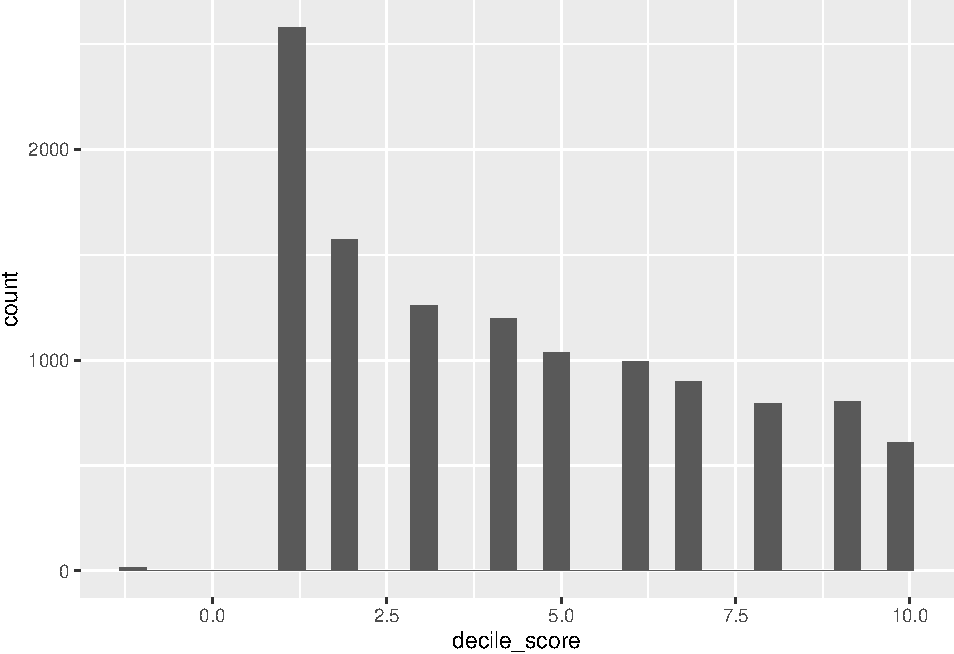
\includegraphics{survival_files/figure-latex/compas-1.pdf}

\begin{Shaded}
\begin{Highlighting}[]
\FunctionTok{table}\NormalTok{(}\SpecialCharTok{!}\FunctionTok{is.na}\NormalTok{(dat}\SpecialCharTok{$}\NormalTok{decile\_score))}
\end{Highlighting}
\end{Shaded}

\begin{verbatim}
## 
##  TRUE 
## 11757
\end{verbatim}

General recommendations:

\begin{itemize}
\item
  Look at the raw data and different plots of the data before doing any
  modeling.
\item
  Look for missing data and for values that might not make sense.
\item
  Make sure you understand what observations (rows) are included in the
  data and which of those observations serve your data analysis goals
\item
  Try to understand what the variables (columns) represent and which
  ones will serve your data analysis goals
\end{itemize}

\hypertarget{quantifying-racial-bias}{%
\subsection{Quantifying racial bias}\label{quantifying-racial-bias}}

\begin{itemize}
\tightlist
\item
  Before doing any analysis, let's look at recidivism, COMPAS, and race
\end{itemize}

\begin{Shaded}
\begin{Highlighting}[]
\NormalTok{df }\OtherTok{\textless{}{-}}\NormalTok{ dat[dat}\SpecialCharTok{$}\NormalTok{is\_recid }\SpecialCharTok{!=} \SpecialCharTok{{-}}\DecValTok{1}\NormalTok{,]}
\FunctionTok{sum}\NormalTok{(}\FunctionTok{is.na}\NormalTok{(df}\SpecialCharTok{$}\NormalTok{race))}
\end{Highlighting}
\end{Shaded}

\begin{verbatim}
## [1] 0
\end{verbatim}

\begin{Shaded}
\begin{Highlighting}[]
\FunctionTok{sum}\NormalTok{(}\FunctionTok{is.na}\NormalTok{(df}\SpecialCharTok{$}\NormalTok{is\_recid))}
\end{Highlighting}
\end{Shaded}

\begin{verbatim}
## [1] 0
\end{verbatim}

\begin{Shaded}
\begin{Highlighting}[]
\FunctionTok{table}\NormalTok{(df}\SpecialCharTok{$}\NormalTok{race, df}\SpecialCharTok{$}\NormalTok{is\_recid)[,}\DecValTok{2}\NormalTok{]}\SpecialCharTok{/}\FunctionTok{t}\NormalTok{(}\FunctionTok{table}\NormalTok{(df}\SpecialCharTok{$}\NormalTok{race))}\SpecialCharTok{*}\DecValTok{100}
\end{Highlighting}
\end{Shaded}

\begin{verbatim}
##       
##        African-American    Asian Caucasian Hispanic Native American    Other
##   [1,]         39.53827 20.75472  28.52279 25.86720        36.11111 24.79871
\end{verbatim}

Above is the recidivism rate by race

\begin{itemize}
\tightlist
\item
  COMPAS also gave Black Americans greater scores on average:
\end{itemize}

\begin{Shaded}
\begin{Highlighting}[]
\FunctionTok{tapply}\NormalTok{(df}\SpecialCharTok{$}\NormalTok{decile\_score, df}\SpecialCharTok{$}\NormalTok{race, mean)}
\end{Highlighting}
\end{Shaded}

\begin{verbatim}
## African-American            Asian        Caucasian         Hispanic 
##         5.326850         2.735849         3.647459         3.313181 
##  Native American            Other 
##         4.805556         2.813205
\end{verbatim}

Is this the best way to present this information?

\hypertarget{how-to-model-algorithmic-bias}{%
\subsection{How to model algorithmic
bias?}\label{how-to-model-algorithmic-bias}}

\begin{itemize}
\item
  What does bias mean here?
\item
  Would COMPAS give someone a greater score solely due to being Black or
  some other demographic, without changing anything else?
\item
  Stated differently, if two people have the same risk of recidivism,
  with race being their only difference, will the algorithm score them
  differently
\item
  Remember COMPAS doesn't ask for race directly
\item
  What does race affecting recidivism mean?

  \begin{itemize}
  \tightlist
  \item
    Incorrect: Someones race affects their behavior
  \item
    Correct: The effect of race living in a racially biased society
  \end{itemize}
\item
  How could we quantify bias in this case? Are race and COMPAS still
  associated after taking recidivism into account?
\item
  It is tempting to use
  \texttt{decile\_score\ \textasciitilde{}\ is\_recid\ +\ race}

  \begin{itemize}
  \tightlist
  \item
    This regression could answer the following: Is race helpful for
    predicting COMPAS score while controlling for recidivism?
  \item
    If race were significant, that would indicate that race contributes
    to COMPAS beyond recidivism itself, so COMPAS would be racially
    biased
  \item
    But, this is not a valid model because \texttt{decile\_score} is
    collected before \texttt{is\_recid}
  \end{itemize}
\end{itemize}

\hypertarget{causation-and-collider-bias}{%
\subsection{Causation and Collider
Bias}\label{causation-and-collider-bias}}

\begin{figure}
\centering
\includegraphics{https://imgs.xkcd.com/comics/correlation.png}
\caption{XKCD causal comic}
\end{figure}

\hypertarget{bayesian-network-1}{%
\subsubsection{Bayesian Network 1:}\label{bayesian-network-1}}

\begin{verbatim}
## PhantomJS not found. You can install it with webshot::install_phantomjs(). If it is installed, please make sure the phantomjs executable can be found via the PATH variable.
\end{verbatim}

\hypertarget{htmlwidget-3ea9a80d501e9cc59060}{}
\begin{grViz}

\end{grViz}

Mental Model: Think of a dataset where \(A,B,C\) are collected

\begin{itemize}
\tightlist
\item
  \(A\) = Alcohol
\item
  \(B\) = Hangover
\item
  \(C\) = Miss Class
\end{itemize}

Question: What would a regression model of
\texttt{C\ \textasciitilde{}\ A\ +\ B} yield?

\begin{itemize}
\item
  \begin{enumerate}
  \def\labelenumi{\alph{enumi})}
  \tightlist
  \item
    Both \(A\) and \(B\) should be statistically significant
  \end{enumerate}
\item
  \begin{enumerate}
  \def\labelenumi{\alph{enumi})}
  \setcounter{enumi}{1}
  \tightlist
  \item
    Only \(A\) should be statistically significant
  \end{enumerate}
\item
  \begin{enumerate}
  \def\labelenumi{\alph{enumi})}
  \setcounter{enumi}{2}
  \tightlist
  \item
    Only \(B\) should be statistically significant
  \end{enumerate}
\item
  \begin{enumerate}
  \def\labelenumi{\alph{enumi})}
  \setcounter{enumi}{3}
  \tightlist
  \item
    Neither \(A\) nor \(B\) should be statistically significant
  \end{enumerate}
\end{itemize}

\begin{Shaded}
\begin{Highlighting}[]
\FunctionTok{set.seed}\NormalTok{(}\DecValTok{1234}\NormalTok{)}
\NormalTok{size }\OtherTok{\textless{}{-}} \DecValTok{1000}
\NormalTok{A }\OtherTok{\textless{}{-}} \DecValTok{6}\SpecialCharTok{*}\FunctionTok{rnorm}\NormalTok{(size)}\SpecialCharTok{+}\DecValTok{50}
\NormalTok{B }\OtherTok{\textless{}{-}} \SpecialCharTok{{-}}\DecValTok{2}\SpecialCharTok{*}\NormalTok{A }\SpecialCharTok{{-}} \DecValTok{25} \SpecialCharTok{+} \FunctionTok{rnorm}\NormalTok{(size)}
\NormalTok{C }\OtherTok{\textless{}{-}} \DecValTok{5}\SpecialCharTok{*}\NormalTok{B }\SpecialCharTok{+} \DecValTok{3} \SpecialCharTok{+}\FunctionTok{rnorm}\NormalTok{(size)}
\FunctionTok{summary}\NormalTok{(}\FunctionTok{lm}\NormalTok{(C}\SpecialCharTok{\textasciitilde{}}\NormalTok{A}\SpecialCharTok{+}\NormalTok{B))}
\end{Highlighting}
\end{Shaded}

\begin{verbatim}
## 
## Call:
## lm(formula = C ~ A + B)
## 
## Residuals:
##      Min       1Q   Median       3Q      Max 
## -3.13161 -0.71957  0.03478  0.70215  3.05316 
## 
## Coefficients:
##             Estimate Std. Error t value Pr(>|t|)    
## (Intercept)  1.96001    0.87456   2.241   0.0252 *  
## A           -0.07084    0.06532  -1.085   0.2784    
## B            4.96310    0.03270 151.761   <2e-16 ***
## ---
## Signif. codes:  0 '***' 0.001 '**' 0.01 '*' 0.05 '.' 0.1 ' ' 1
## 
## Residual standard error: 1.013 on 997 degrees of freedom
## Multiple R-squared:  0.9997, Adjusted R-squared:  0.9997 
## F-statistic: 1.739e+06 on 2 and 997 DF,  p-value: < 2.2e-16
\end{verbatim}

Question: What about this regression model:
\texttt{C\ \textasciitilde{}\ A}?

\begin{itemize}
\item
  \begin{enumerate}
  \def\labelenumi{\alph{enumi})}
  \tightlist
  \item
    \(A\) should be statistically significant
  \end{enumerate}
\item
  \begin{enumerate}
  \def\labelenumi{\alph{enumi})}
  \setcounter{enumi}{1}
  \tightlist
  \item
    \(A\) should not be statistically significant
  \end{enumerate}
\end{itemize}

\begin{Shaded}
\begin{Highlighting}[]
\FunctionTok{summary}\NormalTok{(}\FunctionTok{lm}\NormalTok{(C}\SpecialCharTok{\textasciitilde{}}\NormalTok{A))}
\end{Highlighting}
\end{Shaded}

\begin{verbatim}
## 
## Call:
## lm(formula = C ~ A)
## 
## Residuals:
##      Min       1Q   Median       3Q      Max 
## -15.9753  -3.4048  -0.0059   3.2714  16.5278 
## 
## Coefficients:
##               Estimate Std. Error t value Pr(>|t|)    
## (Intercept) -124.34246    1.31868  -94.29   <2e-16 ***
## A             -9.95096    0.02627 -378.80   <2e-16 ***
## ---
## Signif. codes:  0 '***' 0.001 '**' 0.01 '*' 0.05 '.' 0.1 ' ' 1
## 
## Residual standard error: 4.969 on 998 degrees of freedom
## Multiple R-squared:  0.9931, Adjusted R-squared:  0.9931 
## F-statistic: 1.435e+05 on 1 and 998 DF,  p-value: < 2.2e-16
\end{verbatim}

\begin{itemize}
\tightlist
\item
  Coefficient estimates: \[\begin{align}
  C &= 5B + 3 + \epsilon_B \\
  &= 5(-2A - 25 + \epsilon_A) + 3 + \epsilon_B \\
  &= -10A - 122 + 5\epsilon_A + \epsilon_B
  \end{align}\]
\end{itemize}

Question: Does this coefficient and intercept estimate make sense?

\begin{itemize}
\item
  \begin{enumerate}
  \def\labelenumi{\alph{enumi})}
  \tightlist
  \item
    yes
  \end{enumerate}
\item
  \begin{enumerate}
  \def\labelenumi{\alph{enumi})}
  \setcounter{enumi}{1}
  \tightlist
  \item
    nope
  \end{enumerate}
\end{itemize}

\hypertarget{bayesian-network-2}{%
\subsubsection{Bayesian Network 2:}\label{bayesian-network-2}}

\hypertarget{htmlwidget-957489eae0dd679f4e25}{}
\begin{grViz}

\end{grViz}

Mental Model:

\begin{itemize}
\tightlist
\item
  \(A\) = Smoker
\item
  \(B\) = Yellow Teeth
\item
  \(C\) = Cancer
\end{itemize}

Question: What would a regression model of
\texttt{C\ \textasciitilde{}\ A\ +\ B} yield?

\begin{itemize}
\item
  \begin{enumerate}
  \def\labelenumi{\alph{enumi})}
  \tightlist
  \item
    Both \(A\) and \(B\) should be statistically significant
  \end{enumerate}
\item
  \begin{enumerate}
  \def\labelenumi{\alph{enumi})}
  \setcounter{enumi}{1}
  \tightlist
  \item
    Only \(A\) should be statistically significant
  \end{enumerate}
\item
  \begin{enumerate}
  \def\labelenumi{\alph{enumi})}
  \setcounter{enumi}{2}
  \tightlist
  \item
    Only \(B\) should be statistically significant
  \end{enumerate}
\item
  \begin{enumerate}
  \def\labelenumi{\alph{enumi})}
  \setcounter{enumi}{3}
  \tightlist
  \item
    Neither \(A\) nor \(B\) should be statistically significant
  \end{enumerate}
\end{itemize}

\begin{Shaded}
\begin{Highlighting}[]
\FunctionTok{set.seed}\NormalTok{(}\DecValTok{1234}\NormalTok{)}
\NormalTok{size }\OtherTok{\textless{}{-}} \DecValTok{1000}
\NormalTok{A }\OtherTok{\textless{}{-}} \DecValTok{6}\SpecialCharTok{*}\FunctionTok{rnorm}\NormalTok{(size)}\SpecialCharTok{+}\DecValTok{50}
\NormalTok{B }\OtherTok{\textless{}{-}} \SpecialCharTok{{-}}\DecValTok{2}\SpecialCharTok{*}\NormalTok{A }\SpecialCharTok{{-}} \DecValTok{25} \SpecialCharTok{+} \FunctionTok{rnorm}\NormalTok{(size)}
\NormalTok{C }\OtherTok{\textless{}{-}} \DecValTok{2}\SpecialCharTok{*}\NormalTok{A }\SpecialCharTok{+}\DecValTok{5} \SpecialCharTok{+}\FunctionTok{rnorm}\NormalTok{(size)}
\FunctionTok{summary}\NormalTok{(}\FunctionTok{lm}\NormalTok{(C}\SpecialCharTok{\textasciitilde{}}\NormalTok{A}\SpecialCharTok{+}\NormalTok{B))}
\end{Highlighting}
\end{Shaded}

\begin{verbatim}
## 
## Call:
## lm(formula = C ~ A + B)
## 
## Residuals:
##      Min       1Q   Median       3Q      Max 
## -3.13161 -0.71957  0.03478  0.70215  3.05316 
## 
## Coefficients:
##             Estimate Std. Error t value Pr(>|t|)    
## (Intercept)  3.96001    0.87456   4.528 6.67e-06 ***
## A            1.92916    0.06532  29.533  < 2e-16 ***
## B           -0.03690    0.03270  -1.128    0.259    
## ---
## Signif. codes:  0 '***' 0.001 '**' 0.01 '*' 0.05 '.' 0.1 ' ' 1
## 
## Residual standard error: 1.013 on 997 degrees of freedom
## Multiple R-squared:  0.9929, Adjusted R-squared:  0.9929 
## F-statistic: 6.996e+04 on 2 and 997 DF,  p-value: < 2.2e-16
\end{verbatim}

Question: What about this regression model:
\texttt{C\ \textasciitilde{}\ A}?

\begin{itemize}
\item
  \begin{enumerate}
  \def\labelenumi{\alph{enumi})}
  \tightlist
  \item
    \(A\) should be statistically significant
  \end{enumerate}
\item
  \begin{enumerate}
  \def\labelenumi{\alph{enumi})}
  \setcounter{enumi}{1}
  \tightlist
  \item
    \(A\) should not be statistically significant
  \end{enumerate}
\end{itemize}

\hypertarget{bayesian-network-3}{%
\subsubsection{Bayesian Network 3:}\label{bayesian-network-3}}

\hypertarget{htmlwidget-b338999871153722f361}{}
\begin{grViz}

\end{grViz}

Mental Model:

\begin{itemize}
\tightlist
\item
  \(A\) = Allergies
\item
  \(B\) = Flu
\item
  \(C\) = Sinus
\end{itemize}

Question: What would a regression model of
\texttt{C\ \textasciitilde{}\ A\ +\ B} yield?

\begin{itemize}
\item
  \begin{enumerate}
  \def\labelenumi{\alph{enumi})}
  \tightlist
  \item
    Both \(A\) and \(B\) should be statistically significant
  \end{enumerate}
\item
  \begin{enumerate}
  \def\labelenumi{\alph{enumi})}
  \setcounter{enumi}{1}
  \tightlist
  \item
    Only \(A\) should be statistically significant
  \end{enumerate}
\item
  \begin{enumerate}
  \def\labelenumi{\alph{enumi})}
  \setcounter{enumi}{2}
  \tightlist
  \item
    Only \(B\) should be statistically significant
  \end{enumerate}
\item
  \begin{enumerate}
  \def\labelenumi{\alph{enumi})}
  \setcounter{enumi}{3}
  \tightlist
  \item
    Neither \(A\) nor \(B\) should be statistically significant
  \end{enumerate}
\end{itemize}

\begin{Shaded}
\begin{Highlighting}[]
\FunctionTok{set.seed}\NormalTok{(}\DecValTok{1234}\NormalTok{)}
\NormalTok{size }\OtherTok{\textless{}{-}} \DecValTok{1000}
\NormalTok{A }\OtherTok{\textless{}{-}} \DecValTok{6}\SpecialCharTok{*}\FunctionTok{rnorm}\NormalTok{(size)}\SpecialCharTok{+}\DecValTok{50}
\NormalTok{B }\OtherTok{\textless{}{-}} \SpecialCharTok{{-}}\DecValTok{2}\SpecialCharTok{*}\FunctionTok{rnorm}\NormalTok{(size) }\SpecialCharTok{{-}} \DecValTok{25} \SpecialCharTok{+} \FunctionTok{rnorm}\NormalTok{(size)}
\NormalTok{C }\OtherTok{\textless{}{-}} \SpecialCharTok{{-}}\DecValTok{4}\SpecialCharTok{*}\NormalTok{A }\SpecialCharTok{+} \DecValTok{5}\SpecialCharTok{*}\NormalTok{B }\SpecialCharTok{+} \DecValTok{3} \SpecialCharTok{+}\FunctionTok{rnorm}\NormalTok{(size)}
\FunctionTok{summary}\NormalTok{(}\FunctionTok{lm}\NormalTok{(C}\SpecialCharTok{\textasciitilde{}}\NormalTok{A}\SpecialCharTok{+}\NormalTok{B))}
\end{Highlighting}
\end{Shaded}

\begin{verbatim}
## 
## Call:
## lm(formula = C ~ A + B)
## 
## Residuals:
##      Min       1Q   Median       3Q      Max 
## -3.03321 -0.68565  0.01655  0.66794  3.13811 
## 
## Coefficients:
##              Estimate Std. Error  t value Pr(>|t|)    
## (Intercept)  2.967859   0.430869    6.888    1e-11 ***
## A           -4.000487   0.005264 -759.946   <2e-16 ***
## B            4.998128   0.014068  355.283   <2e-16 ***
## ---
## Signif. codes:  0 '***' 0.001 '**' 0.01 '*' 0.05 '.' 0.1 ' ' 1
## 
## Residual standard error: 0.9947 on 997 degrees of freedom
## Multiple R-squared:  0.9986, Adjusted R-squared:  0.9986 
## F-statistic: 3.641e+05 on 2 and 997 DF,  p-value: < 2.2e-16
\end{verbatim}

\hypertarget{bayesian-network-3-again-with-a-as-the-outcome}{%
\subsubsection{\texorpdfstring{Bayesian Network 3 (again) with
\texttt{A} as the
outcome:}{Bayesian Network 3 (again) with A as the outcome:}}\label{bayesian-network-3-again-with-a-as-the-outcome}}

\hypertarget{htmlwidget-35db85c5527a6bd5601b}{}
\begin{grViz}

\end{grViz}

Question: What would a regression model of
\texttt{A\ \textasciitilde{}\ B\ +\ C} yield?

\begin{itemize}
\item
  \begin{enumerate}
  \def\labelenumi{\alph{enumi})}
  \tightlist
  \item
    Both \(B\) and \(C\) should be statistically significant
  \end{enumerate}
\item
  \begin{enumerate}
  \def\labelenumi{\alph{enumi})}
  \setcounter{enumi}{1}
  \tightlist
  \item
    Only \(B\) should be statistically significant
  \end{enumerate}
\item
  \begin{enumerate}
  \def\labelenumi{\alph{enumi})}
  \setcounter{enumi}{2}
  \tightlist
  \item
    Only \(C\) should be statistically significant
  \end{enumerate}
\item
  \begin{enumerate}
  \def\labelenumi{\alph{enumi})}
  \setcounter{enumi}{3}
  \tightlist
  \item
    Neither \(B\) nor \(C\) should be statistically significant
  \end{enumerate}
\end{itemize}

\begin{Shaded}
\begin{Highlighting}[]
\FunctionTok{summary}\NormalTok{(}\FunctionTok{lm}\NormalTok{(A}\SpecialCharTok{\textasciitilde{}}\NormalTok{B}\SpecialCharTok{+}\NormalTok{C))}
\end{Highlighting}
\end{Shaded}

\begin{verbatim}
## 
## Call:
## lm(formula = A ~ B + C)
## 
## Residuals:
##      Min       1Q   Median       3Q      Max 
## -0.75638 -0.17022  0.00544  0.16841  0.80335 
## 
## Coefficients:
##               Estimate Std. Error  t value Pr(>|t|)    
## (Intercept)  0.8215779  0.1070244    7.677 3.89e-14 ***
## B            1.2470301  0.0039408  316.439  < 2e-16 ***
## C           -0.2495388  0.0003284 -759.946  < 2e-16 ***
## ---
## Signif. codes:  0 '***' 0.001 '**' 0.01 '*' 0.05 '.' 0.1 ' ' 1
## 
## Residual standard error: 0.2484 on 997 degrees of freedom
## Multiple R-squared:  0.9983, Adjusted R-squared:  0.9983 
## F-statistic: 2.893e+05 on 2 and 997 DF,  p-value: < 2.2e-16
\end{verbatim}

Question: What would a regression model of
\texttt{A\ \textasciitilde{}\ B} yield?

\begin{itemize}
\item
  \begin{enumerate}
  \def\labelenumi{\alph{enumi})}
  \tightlist
  \item
    \(B\) should be statistically significant
  \end{enumerate}
\item
  \begin{enumerate}
  \def\labelenumi{\alph{enumi})}
  \setcounter{enumi}{1}
  \tightlist
  \item
    \(B\) should not be statistically significant
  \end{enumerate}
\end{itemize}

\begin{Shaded}
\begin{Highlighting}[]
\FunctionTok{summary}\NormalTok{(}\FunctionTok{lm}\NormalTok{(A}\SpecialCharTok{\textasciitilde{}}\NormalTok{B))}
\end{Highlighting}
\end{Shaded}

\begin{verbatim}
## 
## Call:
## lm(formula = A ~ B)
## 
## Residuals:
##      Min       1Q   Median       3Q      Max 
## -19.9644  -3.8309  -0.0804   3.8547  19.3418 
## 
## Coefficients:
##             Estimate Std. Error t value Pr(>|t|)    
## (Intercept) 46.99023    2.12137  22.151   <2e-16 ***
## B           -0.11401    0.08452  -1.349    0.178    
## ---
## Signif. codes:  0 '***' 0.001 '**' 0.01 '*' 0.05 '.' 0.1 ' ' 1
## 
## Residual standard error: 5.982 on 998 degrees of freedom
## Multiple R-squared:  0.00182,    Adjusted R-squared:  0.0008198 
## F-statistic:  1.82 on 1 and 998 DF,  p-value: 0.1777
\end{verbatim}

\begin{itemize}
\item
  Even though \texttt{A} and \texttt{B} are independent, they are
  \emph{conditionally dependent} if controlling for \texttt{C}.
\item
  Why did this happen? Let's take a simple example
\item
  Assume \(A\sim \text{Bernoulli}(0.4)\), and
  \(B\sim \text{Bernoulli}(0.7)\)
\item
  Question: What is \(P(B=1|A=1)\)?
\item
  Define
  \(C = \begin{cases} 1 \text{ when } A=B \\ 0 \text{ when } A\neq B\end{cases}\)
\item
  Question: What is \(P(B=1| A=1, C=0)\)?
\item
  \(A\) and \(B\) are independent; that is, knowledge of \(B\) give no
  information on the value of \(A\). But, additional knowledge of \(C\)
  does give information about the value of \(A\).
\end{itemize}

\textbf{Bayesian Network 4}

\hypertarget{htmlwidget-35e18a5c42075fe63654}{}
\begin{grViz}

\end{grViz}

Mental Model:

\begin{itemize}
\tightlist
\item
  \(A\) = Study into the night
\item
  \(B\) = Go to bed late
\item
  \(C\) = Fail Test
\end{itemize}

Question: What would a regression model of
\texttt{C\ \textasciitilde{}\ A\ +\ B} yield?

\begin{itemize}
\item
  \begin{enumerate}
  \def\labelenumi{\alph{enumi})}
  \tightlist
  \item
    Both \(A\) and \(B\) should be statistically significant
  \end{enumerate}
\item
  \begin{enumerate}
  \def\labelenumi{\alph{enumi})}
  \setcounter{enumi}{1}
  \tightlist
  \item
    Only \(A\) should be statistically significant
  \end{enumerate}
\item
  \begin{enumerate}
  \def\labelenumi{\alph{enumi})}
  \setcounter{enumi}{2}
  \tightlist
  \item
    Only \(B\) should be statistically significant
  \end{enumerate}
\item
  \begin{enumerate}
  \def\labelenumi{\alph{enumi})}
  \setcounter{enumi}{3}
  \tightlist
  \item
    Neither \(A\) nor \(B\) should be statistically significant
  \end{enumerate}
\end{itemize}

\begin{Shaded}
\begin{Highlighting}[]
\FunctionTok{set.seed}\NormalTok{(}\DecValTok{1234}\NormalTok{)}
\NormalTok{size }\OtherTok{\textless{}{-}} \DecValTok{1000}
\NormalTok{A }\OtherTok{\textless{}{-}} \DecValTok{6}\SpecialCharTok{*}\FunctionTok{rnorm}\NormalTok{(size)}\SpecialCharTok{+}\DecValTok{50}
\NormalTok{B }\OtherTok{\textless{}{-}}\NormalTok{ A }\SpecialCharTok{{-}} \DecValTok{25} \SpecialCharTok{{-}} \DecValTok{2}\SpecialCharTok{*}\FunctionTok{rnorm}\NormalTok{(size)}
\NormalTok{C }\OtherTok{\textless{}{-}} \SpecialCharTok{{-}}\DecValTok{4}\SpecialCharTok{*}\NormalTok{A }\SpecialCharTok{+} \DecValTok{5}\SpecialCharTok{*}\NormalTok{B }\SpecialCharTok{+} \DecValTok{3} \SpecialCharTok{+}\FunctionTok{rnorm}\NormalTok{(size)}
\FunctionTok{summary}\NormalTok{(}\FunctionTok{lm}\NormalTok{(C}\SpecialCharTok{\textasciitilde{}}\NormalTok{A}\SpecialCharTok{+}\NormalTok{B))}
\end{Highlighting}
\end{Shaded}

\begin{verbatim}
## 
## Call:
## lm(formula = C ~ A + B)
## 
## Residuals:
##      Min       1Q   Median       3Q      Max 
## -3.13161 -0.71957  0.03478  0.70215  3.05316 
## 
## Coefficients:
##             Estimate Std. Error  t value Pr(>|t|)    
## (Intercept)  3.34366    0.47704    7.009 4.41e-12 ***
## A           -4.01550    0.01692 -237.358  < 2e-16 ***
## B            5.01845    0.01635  306.907  < 2e-16 ***
## ---
## Signif. codes:  0 '***' 0.001 '**' 0.01 '*' 0.05 '.' 0.1 ' ' 1
## 
## Residual standard error: 1.013 on 997 degrees of freedom
## Multiple R-squared:  0.992,  Adjusted R-squared:  0.9919 
## F-statistic: 6.153e+04 on 2 and 997 DF,  p-value: < 2.2e-16
\end{verbatim}

Question: What about this regression model:
\texttt{C\ \textasciitilde{}\ A}?

\begin{itemize}
\item
  \begin{enumerate}
  \def\labelenumi{\alph{enumi})}
  \tightlist
  \item
    \(A\) should be statistically significant
  \end{enumerate}
\item
  \begin{enumerate}
  \def\labelenumi{\alph{enumi})}
  \setcounter{enumi}{1}
  \tightlist
  \item
    \(A\) should not be statistically significant
  \end{enumerate}
\end{itemize}

\begin{Shaded}
\begin{Highlighting}[]
\FunctionTok{summary}\NormalTok{(}\FunctionTok{lm}\NormalTok{(C}\SpecialCharTok{\textasciitilde{}}\NormalTok{A))}
\end{Highlighting}
\end{Shaded}

\begin{verbatim}
## 
## Call:
## lm(formula = C ~ A)
## 
## Residuals:
##      Min       1Q   Median       3Q      Max 
## -30.7632  -6.7266  -0.2299   6.3962  31.5156 
## 
## Coefficients:
##               Estimate Std. Error t value Pr(>|t|)    
## (Intercept) -117.61814    2.62464  -44.81   <2e-16 ***
## A              0.90975    0.05229   17.40   <2e-16 ***
## ---
## Signif. codes:  0 '***' 0.001 '**' 0.01 '*' 0.05 '.' 0.1 ' ' 1
## 
## Residual standard error: 9.889 on 998 degrees of freedom
## Multiple R-squared:  0.2327, Adjusted R-squared:  0.232 
## F-statistic: 302.7 on 1 and 998 DF,  p-value: < 2.2e-16
\end{verbatim}

Question: What about this regression model:
\texttt{B\ \textasciitilde{}\ A\ +\ C}?

\begin{itemize}
\item
  \begin{enumerate}
  \def\labelenumi{\alph{enumi})}
  \tightlist
  \item
    Both \(A\) and \(C\) should be statistically significant
  \end{enumerate}
\item
  \begin{enumerate}
  \def\labelenumi{\alph{enumi})}
  \setcounter{enumi}{1}
  \tightlist
  \item
    Only \(A\) should be statistically significant
  \end{enumerate}
\item
  \begin{enumerate}
  \def\labelenumi{\alph{enumi})}
  \setcounter{enumi}{2}
  \tightlist
  \item
    Only \(C\) should be statistically significant
  \end{enumerate}
\item
  \begin{enumerate}
  \def\labelenumi{\alph{enumi})}
  \setcounter{enumi}{3}
  \tightlist
  \item
    Neither \(A\) nor \(C\) should be statistically significant
  \end{enumerate}
\end{itemize}

\begin{Shaded}
\begin{Highlighting}[]
\FunctionTok{summary}\NormalTok{(}\FunctionTok{lm}\NormalTok{(B}\SpecialCharTok{\textasciitilde{}}\NormalTok{A}\SpecialCharTok{+}\NormalTok{C))}
\end{Highlighting}
\end{Shaded}

\begin{verbatim}
## 
## Call:
## lm(formula = B ~ A + C)
## 
## Residuals:
##      Min       1Q   Median       3Q      Max 
## -0.61703 -0.13791 -0.00305  0.14136  0.62353 
## 
## Coefficients:
##               Estimate Std. Error t value Pr(>|t|)    
## (Intercept) -0.9117518  0.0924550  -9.862   <2e-16 ***
## A            0.8020461  0.0012115 662.016   <2e-16 ***
## C            0.1971777  0.0006425 306.907   <2e-16 ***
## ---
## Signif. codes:  0 '***' 0.001 '**' 0.01 '*' 0.05 '.' 0.1 ' ' 1
## 
## Residual standard error: 0.2007 on 997 degrees of freedom
## Multiple R-squared:  0.999,  Adjusted R-squared:  0.9989 
## F-statistic: 4.747e+05 on 2 and 997 DF,  p-value: < 2.2e-16
\end{verbatim}

\hypertarget{compas-and-possible-collider-bias}{%
\subsection{COMPAS and possible collider
bias}\label{compas-and-possible-collider-bias}}

\begin{itemize}
\item
  COMPAS uses
  \href{https://www.documentcloud.org/documents/2702103-Sample-Risk-Assessment-COMPAS-CORE.html}{questionnaire}
  responses to predict recidivism.
\item
  Because COMPAS is used in sentencing, it may actually impact
  recidivism as well.
\item
  One way to quantify racial bias in COMPAS would be to isolate the link
  between race and COMPAS that is not associated with recidivism. But,
  it is not clear how to untangle this from potential collider bias.
\end{itemize}

\begin{Shaded}
\begin{Highlighting}[]
\KeywordTok{digraph} \OtherTok{\{}
\CommentTok{  }\VariableTok{Race}\CommentTok{ }\OtherTok{{-}\textgreater{}}\CommentTok{ }\VariableTok{COMPAS}\CommentTok{ }\OtherTok{[}\CommentTok{ }\AttributeTok{label}\CommentTok{ }\OtherTok{=}\CommentTok{ }\StringTok{"?"}\OtherTok{];}
\CommentTok{  }\VariableTok{COMPAS}\CommentTok{ }\OtherTok{{-}\textgreater{}}\CommentTok{ }\VariableTok{Recidivism}\CommentTok{ }\OtherTok{[}\CommentTok{ }\AttributeTok{label}\CommentTok{ }\OtherTok{=}\CommentTok{ }\StringTok{"?"}\OtherTok{];}\CommentTok{ }
\CommentTok{  }\VariableTok{Race}\CommentTok{ }\OtherTok{{-}\textgreater{}}\CommentTok{ }\VariableTok{Recidivism}\CommentTok{ }\OtherTok{[}\CommentTok{ }\AttributeTok{label}\CommentTok{ }\OtherTok{=}\CommentTok{ }\StringTok{"?"}\OtherTok{]}
\CommentTok{  }\OtherTok{\}}
\end{Highlighting}
\end{Shaded}

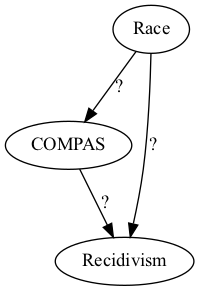
\includegraphics[width=0.4\linewidth]{survival_files/figure-latex/unnamed-chunk-13-1}

\begin{itemize}
\item
  If we used
  \texttt{decile\_score\ \textasciitilde{}\ is\_recid\ +\ race} as a
  model to quantify bias, it seems very likely that there will be
  collider bias
\item
  IMPORTANT: The model below is NOT informative because of the possible
  causal structure of the data

  \begin{itemize}
  \tightlist
  \item
    Included for teaching purposes only
  \end{itemize}
\end{itemize}

\begin{Shaded}
\begin{Highlighting}[]
\FunctionTok{summary}\NormalTok{(}\FunctionTok{lm}\NormalTok{(decile\_score }\SpecialCharTok{\textasciitilde{}}\NormalTok{ is\_recid }\SpecialCharTok{+}\NormalTok{ race, }\AttributeTok{data=}\NormalTok{df))}
\end{Highlighting}
\end{Shaded}

\begin{verbatim}
## 
## Call:
## lm(formula = decile_score ~ is_recid + race, data = df)
## 
## Residuals:
##    Min     1Q Median     3Q    Max 
## -7.225 -2.224 -0.225  1.776  7.555 
## 
## Coefficients:
##                     Estimate Std. Error t value Pr(>|t|)    
## (Intercept)          4.73952    0.04127 114.848  < 2e-16 ***
## is_recid             1.48548    0.05345  27.794  < 2e-16 ***
## raceAsian           -2.31198    0.36300  -6.369 1.98e-10 ***
## raceCaucasian       -1.51576    0.05569 -27.217  < 2e-16 ***
## raceHispanic        -1.81059    0.09033 -20.043  < 2e-16 ***
## raceNative American -0.47038    0.43961  -1.070    0.285    
## raceOther           -2.29469    0.11157 -20.566  < 2e-16 ***
## ---
## Signif. codes:  0 '***' 0.001 '**' 0.01 '*' 0.05 '.' 0.1 ' ' 1
## 
## Residual standard error: 2.629 on 11031 degrees of freedom
## Multiple R-squared:  0.1656, Adjusted R-squared:  0.1652 
## F-statistic: 364.9 on 6 and 11031 DF,  p-value: < 2.2e-16
\end{verbatim}

In the regression above, several race indicator variables are
significant. But, because collider bias is possible here, we
\emph{cannot} conclude that COMPAS is racially biased.

\hypertarget{survival-analysis}{%
\subsection{Survival Analysis}\label{survival-analysis}}

\begin{itemize}
\item
  Survival analysis is a set of statistical methods for modeling the
  time until an event occurs, especially when follow up is not complete
  for each observation.
\item
  Example: Testing a new terminal cancer treatment, participants are
  either given the standard or test treatment. The goal is to prolong
  the patient's life. Each patient is followed until death from cancer.
  During follow up some participants die from cancer but some drop out
  while others might die from something else. Survival analysis allows
  us to use this data even though we do not have events for each
  participant.
\end{itemize}

\textbf{Set up}

\begin{itemize}
\item
  Assume that \(T\) is the time until an event randomly occurs.
\item
  For example, \(T\) might be the duration from cancer treatment until
  remission or death.
\item
  \(T\sim f\)

  \begin{itemize}
  \tightlist
  \item
    That is, \(f(t)\) is the probability density function (pdf) of \(T\)
    where \(t\) is time
  \end{itemize}
\item
  \(F(t)=P(T<t)=\int_0^tf(x)dx\) is cumulative distribution function
  (cdf) of \(T\)
\item
  Survival function: \[S(t)=P(T>t)=1-F(t)\]
\item
  The survival function gives the probability of not having an event
  before time \(t\) (survive until \(t\))
\item
  Hazard function: \[
  \lambda(t) =\lim_{h\rightarrow 0} P(T\leq t+h | T>t) =\lim_{h\rightarrow 0} \frac{P(t<T\leq t+h)}{P(T>t)}= \frac{f(t)}{S(t)} = -\frac{d\log S(t)}{dt}.
  \]
\item
  Hazard function gives the instantaneous probability of an event at
  time \(t\) given survival until time \(t\)
\item
  Notice that \(f(t)=\lambda(t)S(t)\)
\item
  Cumulative hazard function: \[
  \Lambda(t)= \int_0^t\lambda(x)dx=-\int_0^td\log S(x)=-\log S(t).
  \]
\item
  How to get the survival function from the hazard function: \[
  S(t)=\exp[-\Lambda(t)].
  \]
\item
  Side note: If \(\lambda(t)=\lambda\) (constant function), then \(f\)
  is the exponential distribution: \[
  \begin{align*}
  \lambda(t)=\lambda 
  &\Leftrightarrow \Lambda(t)=\lambda t \\
  &\Leftrightarrow S(t)=\exp(-\lambda t) \\
  &\Leftrightarrow f(t)= \lambda(t) S(t) = \lambda\exp(-\lambda t)
  \end{align*}
  \]
\end{itemize}

\textbf{Censoring at Random}

\begin{itemize}
\item
  Not always possible to wait for an event to occur for each participant
  before doing the analysis
\item
  Cancer study example: participants may drop out of the study before an
  event is observed or the study may close before each participant
  experiences an event
\item
  This is call right censored data: have start time but end times can
  either be at event or drop out time
\item
  Question: For censored observations, how to make use of time duration
  without event?
\end{itemize}

\begin{figure}
\centering
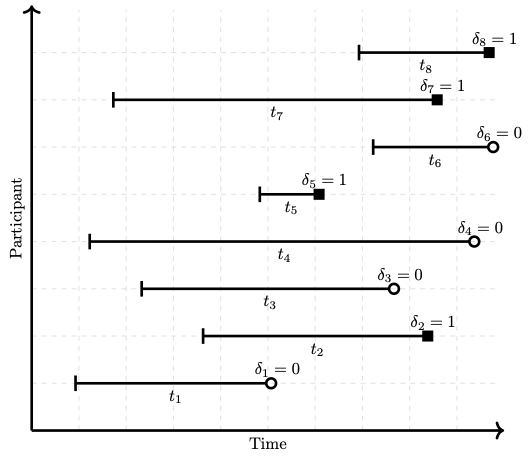
\includegraphics{./censoredData.png}
\caption{Right Censored Data}
\end{figure}

\begin{itemize}
\item
  Model: \(f(t|x; \theta)\) with corresponding hazard,
  \(\lambda(t|x;\theta)\), and survival, \(S(t|x;\theta)\)
\item
  Want \(\theta\) to quantify difference in risk (until event) among
  observations

  \begin{itemize}
  \tightlist
  \item
    Note: \(\theta\) quantifies how fast an event will likely occur for
    an observation but communicated in terms of risk of event
  \end{itemize}
\item
  Assumption: censoring occurs at random (in independently from \(f\))
\item
  Censoring cumulative probability distribution model: \[G(t;\phi)\]
\item
  Corresponding censoring pdf model: \[g(t;\phi)\]
\item
  Data: \[(t_1, \delta_1),\dots, (t_n,\delta_n)\]
\item
  \(t_i\) for \(i=1,\dots,n\) is duration of follow-up until either
  event or censor time
\item
  \(\delta_i\) is event indicator:

  \begin{itemize}
  \tightlist
  \item
    \(\delta_i=1\) means that observation \(i\) had an event and
    \(t_i \sim f(t;\theta)\)
  \item
    \(\delta_i=0\) means that observation \(i\) was censored and
    \(t_i \sim g(t;\phi)\)
  \end{itemize}
\item
  Because \(f\) and \(g\) are independent (and because observations are
  independent), the likelihood is \[
  \begin{align}
  L(\theta,\phi) &= \prod_{i=1}^n [f(t_i;\theta)[1-G(t_i;\phi)]]^{\delta_i} [g(t_i;\phi)S(t_i;\theta)]^{1-\delta_i}\\
  &=  \prod_{i=1}^n [f(t_i;\theta)]^{\delta_i}[S(t_i;\theta)]^{1-\delta_i} \prod_{i=1}^n [g(t_i;\phi)]^{1-\delta_1}[1-G(t_i;\phi)]^{\delta_i}\\
  &= L(\theta) L(\phi) \propto L(\theta).
  \end{align}
  \]
\item
  Observe an event for \(i\) (\(\delta_i=1\)), then \(t_i\sim f\) and
  censoring did not occur prior
  \([f(t_i;\theta)[1-G(t_i;\phi)]]^{\delta_i}\)
\item
  Observe censoring for \(i\) (\(\delta_i=1\)), then \(t_i\sim g\) and
  an event did not occur prior
  \([g(t_i;\phi)S(t_i;\theta)]^{1-\delta_i}\)
\item
  But, we do not care about the censoring distribution, only the time to
  event distribution.
\item
  Partial likelihood
  \[L(\theta)=\prod_{i=1}^n [f(t_i;\theta)]^{\delta_i}[S(t_i;\theta)]^{1-\delta_i}= \prod_{i=1}^n \lambda(t_i)^{\delta_i} S(t_i)\]
\end{itemize}

\hypertarget{kaplan-meier-estimator}{%
\subsection{Kaplan-Meier Estimator}\label{kaplan-meier-estimator}}

\begin{itemize}
\tightlist
\item
  Question: Have you heard of/seen Kaplan-Meier Curves before this?

  \begin{itemize}
  \tightlist
  \item
    A: Yes
  \item
    B: No
  \end{itemize}
\item
  Visualize the percent of population surviving until time \(t\) as
  \(t\) increases
\end{itemize}

\begin{figure}
\centering
\includegraphics{https://cdn.graphpad.com/faq/1747/images/1747d.gif}
\caption{KM Curve Example}
\end{figure}

\begin{itemize}
\item
  Consider estimating survival: \(S(t) = P(T>t)\) from sample
  \((t_1, \delta_1),\dots, (t_n,\delta_n)\)
\item
  Approximate \(S(t)\) as a non-parametric decreasing step function

  \begin{itemize}
  \tightlist
  \item
    \(S(t)\) is proportion of sample that has not experienced an event
    at time \(t\)
  \item
    Problem: If \(i\) censored prior to \(t\), we cannot know if their
    event occurred before or after \(t\)
  \end{itemize}
\item
  Order sample by event times \(t_i\) where \(\delta_i=1\):
  \[t_{(1)}, t_{(2)}, \dots, t_{(J)}\]
\item
  There are only \(J\) sample points in time where events occur
\item
  Recall conditional probability rule \(P(A|B)=\frac{P(A,B)}{P(B)}\)
\item
  Because \(t_{(j)} > t_{(j-1)}\),
  \[S\left(t_{(j)}\right) = P\left(T > t_{(j)}\right) = P\left(T > t_{(j)}, T > t_{(j-1)}\right) = P\left(T > t_{(j)} | T > t_{(j-1)}\right) \times P\left(T > t_{(j-1)}\right)\]
\item
  Repeating \[\begin{align*}
  S\left(t_{(j)}\right) 
  &= P\left(T > t_{(j)} | T > t_{(j-1)}\right) \times P\left(T > t_{(j-1)} | T > t_{(j-2)}\right) \times P\left(T > t_{(j-2)}\right) \\
  &= P\left(T > t_{(j)} | T > t_{(j-1)}\right) \times P\left(T > t_{(j-1)} | T > t_{(j-2)}\right) \times\dots\times P\left(T > t_{(2)} | T > t_{(1)}\right) \times P\left(T > t_{(1)}\right)\\
  \end{align*}\]
\item
  This seems
  \href{https://www.merriam-webster.com/dictionary/tautology}{tautological},
  but it's helpful here because it allows us to include the censored
  observations in the denominator appropriately as \(t\) increases
\item
  For \(j = 1,\dots, J\), the ``instantaneous'' probability of an event
  occurring at time \(t_j\):
  \[\pi_j = P\left(T \leq t_{(j)} | T > t_{(j-1)}\right) = 1-P\left(T > t_{(j)} | T > t_{(j-1)}\right)\]
\item
  Then \[
  S(t_{(j)}) = (1-\pi_j)(1-\pi_{j-1}) \dots (1-\pi_2)(1-\pi_1).
  \]
\item
  Calculate \(\pi_j\):

  \begin{itemize}
  \item
    Let \(n_j = \#\{t_i \geq t_{(j)}\}\) be the number of participants
    who are still at risk (who haven't had an event or been censored) at
    time \(t_{(j)}\)
  \item
    Note: that \(n_j\) decreases as events occur or as they are
    censored.
  \item
    Let \(d_j = \#\{t_i=t_{(j)}, \delta_i=1\}\) be the number of events
    that occur at time \(t_{(j)}\).
  \item
    Maximizes the non-parametric likelihood \[\pi_j = \frac{d_j}{n_j}\]
  \end{itemize}
\item
  So, we can approximate the survival function as \[
  \hat S(t) = \prod_{j=1}^J \left( 1-\frac{d_j}{n_j}\right)^{I(t_{(j)}\leq t)}.
  \]
\item
  Using the delta-method, we can approxmiate the variance of the
  estimated survival function as \[
  \hat V[\hat S(t)] = \hat S(t)^2 \sum_{j: t_{(j)}\leq t} \frac{d_j}{n_j(n_j-d_j)}
  \]
\item
  With the variance, we can run statistical tests
\end{itemize}

This \href{https://www.youtube.com/watch?v=NDgn72ynHcM}{video} clearly
illustrates how to calculate the KM survival function.

\begin{Shaded}
\begin{Highlighting}[]
\FunctionTok{library}\NormalTok{(survival)}

\NormalTok{dat }\OtherTok{\textless{}{-}} \FunctionTok{read.csv}\NormalTok{(}\FunctionTok{url}\NormalTok{(}\StringTok{\textquotesingle{}https://raw.githubusercontent.com/propublica/compas{-}analysis/master/cox{-}parsed.csv\textquotesingle{}}\NormalTok{))}
\FunctionTok{names}\NormalTok{(dat)}
\end{Highlighting}
\end{Shaded}

\begin{verbatim}
##  [1] "id"                      "name"                   
##  [3] "first"                   "last"                   
##  [5] "compas_screening_date"   "sex"                    
##  [7] "dob"                     "age"                    
##  [9] "age_cat"                 "race"                   
## [11] "juv_fel_count"           "decile_score"           
## [13] "juv_misd_count"          "juv_other_count"        
## [15] "priors_count"            "days_b_screening_arrest"
## [17] "c_jail_in"               "c_jail_out"             
## [19] "c_case_number"           "c_offense_date"         
## [21] "c_arrest_date"           "c_days_from_compas"     
## [23] "c_charge_degree"         "c_charge_desc"          
## [25] "is_recid"                "r_case_number"          
## [27] "r_charge_degree"         "r_days_from_arrest"     
## [29] "r_offense_date"          "r_charge_desc"          
## [31] "r_jail_in"               "r_jail_out"             
## [33] "violent_recid"           "is_violent_recid"       
## [35] "vr_case_number"          "vr_charge_degree"       
## [37] "vr_offense_date"         "vr_charge_desc"         
## [39] "type_of_assessment"      "decile_score.1"         
## [41] "score_text"              "screening_date"         
## [43] "v_type_of_assessment"    "v_decile_score"         
## [45] "v_score_text"            "v_screening_date"       
## [47] "in_custody"              "out_custody"            
## [49] "priors_count.1"          "start"                  
## [51] "end"                     "event"
\end{verbatim}

\begin{Shaded}
\begin{Highlighting}[]
\FunctionTok{dim}\NormalTok{(dat)}
\end{Highlighting}
\end{Shaded}

\begin{verbatim}
## [1] 13419    52
\end{verbatim}

\begin{Shaded}
\begin{Highlighting}[]
\NormalTok{dat2 }\OtherTok{\textless{}{-}}\NormalTok{ dat[dat}\SpecialCharTok{$}\NormalTok{end }\SpecialCharTok{\textgreater{}}\NormalTok{ dat}\SpecialCharTok{$}\NormalTok{start,]}
\FunctionTok{dim}\NormalTok{(dat2)}
\end{Highlighting}
\end{Shaded}

\begin{verbatim}
## [1] 13356    52
\end{verbatim}

\begin{Shaded}
\begin{Highlighting}[]
\NormalTok{dat3 }\OtherTok{\textless{}{-}}\NormalTok{ dat2[}\SpecialCharTok{!}\FunctionTok{duplicated}\NormalTok{(dat2}\SpecialCharTok{$}\NormalTok{id),]}
\FunctionTok{dim}\NormalTok{(dat3)}
\end{Highlighting}
\end{Shaded}

\begin{verbatim}
## [1] 10325    52
\end{verbatim}

\begin{Shaded}
\begin{Highlighting}[]
\NormalTok{ph }\OtherTok{\textless{}{-}}\NormalTok{ dat3[dat3}\SpecialCharTok{$}\NormalTok{decile\_score}\SpecialCharTok{\textgreater{}}\DecValTok{0}\NormalTok{,]}
\FunctionTok{dim}\NormalTok{(ph)}
\end{Highlighting}
\end{Shaded}

\begin{verbatim}
## [1] 10314    52
\end{verbatim}

\begin{Shaded}
\begin{Highlighting}[]
\NormalTok{ph}\SpecialCharTok{$}\NormalTok{t\_atrisk }\OtherTok{\textless{}{-}}\NormalTok{ ph}\SpecialCharTok{$}\NormalTok{end }\SpecialCharTok{{-}}\NormalTok{ ph}\SpecialCharTok{$}\NormalTok{start}

\NormalTok{survobj }\OtherTok{\textless{}{-}} \FunctionTok{with}\NormalTok{(ph, }\FunctionTok{Surv}\NormalTok{(t\_atrisk, event))}
\NormalTok{fit0 }\OtherTok{\textless{}{-}} \FunctionTok{survfit}\NormalTok{(survobj}\SpecialCharTok{\textasciitilde{}}\DecValTok{1}\NormalTok{, }\AttributeTok{data=}\NormalTok{ph)}
\CommentTok{\# summary(fit0)}
\FunctionTok{plot}\NormalTok{(fit0, }\AttributeTok{xlab=}\StringTok{"Time at risk of recidivism in Days"}\NormalTok{, }
   \AttributeTok{ylab=}\StringTok{"\% not rearrested"}\NormalTok{, }\AttributeTok{yscale=}\DecValTok{100}\NormalTok{,}
   \AttributeTok{main =}\StringTok{"Survival Distribution (Overall)"}\NormalTok{) }
\end{Highlighting}
\end{Shaded}

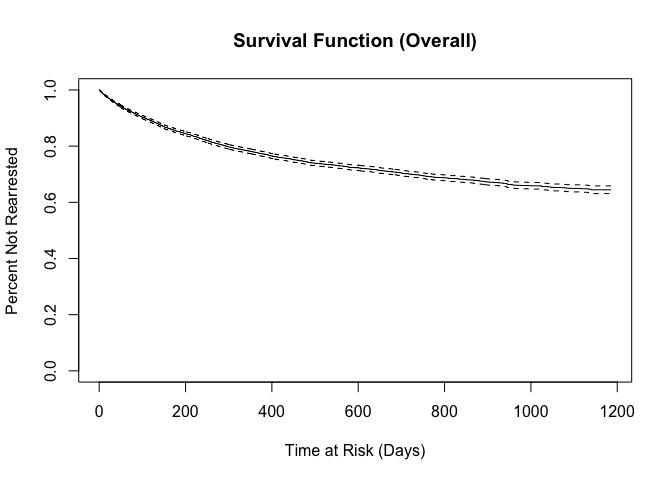
\includegraphics{survival_files/figure-latex/km_curve-1.pdf}

\begin{Shaded}
\begin{Highlighting}[]
\NormalTok{fitr }\OtherTok{\textless{}{-}} \FunctionTok{survfit}\NormalTok{(survobj}\SpecialCharTok{\textasciitilde{}}\NormalTok{race, }\AttributeTok{data=}\NormalTok{ph)}
\FunctionTok{plot}\NormalTok{(fitr, }\AttributeTok{xlab=}\StringTok{"Time at risk of recidivism in Days"}\NormalTok{, }
   \AttributeTok{ylab=}\StringTok{"\% not rearrested"}\NormalTok{, }\AttributeTok{yscale=}\DecValTok{100}\NormalTok{,}
   \AttributeTok{main=}\StringTok{"Survival Distribution by race"}\NormalTok{,}
   \AttributeTok{col =} \FunctionTok{c}\NormalTok{(}\StringTok{\textquotesingle{}red\textquotesingle{}}\NormalTok{, }\StringTok{\textquotesingle{}blue\textquotesingle{}}\NormalTok{, }\StringTok{\textquotesingle{}orange\textquotesingle{}}\NormalTok{, }\StringTok{\textquotesingle{}yellow\textquotesingle{}}\NormalTok{, }\StringTok{\textquotesingle{}green\textquotesingle{}}\NormalTok{, }\StringTok{\textquotesingle{}purple\textquotesingle{}}\NormalTok{)) }
\FunctionTok{legend}\NormalTok{(}\StringTok{\textquotesingle{}bottomleft\textquotesingle{}}\NormalTok{, }\AttributeTok{legend=}\FunctionTok{levels}\NormalTok{(}\FunctionTok{as.factor}\NormalTok{(ph}\SpecialCharTok{$}\NormalTok{race)), }\AttributeTok{col =} \FunctionTok{c}\NormalTok{(}\StringTok{\textquotesingle{}red\textquotesingle{}}\NormalTok{, }\StringTok{\textquotesingle{}blue\textquotesingle{}}\NormalTok{, }\StringTok{\textquotesingle{}orange\textquotesingle{}}\NormalTok{, }\StringTok{\textquotesingle{}yellow\textquotesingle{}}\NormalTok{, }\StringTok{\textquotesingle{}green\textquotesingle{}}\NormalTok{, }\StringTok{\textquotesingle{}purple\textquotesingle{}}\NormalTok{), }\AttributeTok{lty=}\DecValTok{1}\NormalTok{)}
\end{Highlighting}
\end{Shaded}

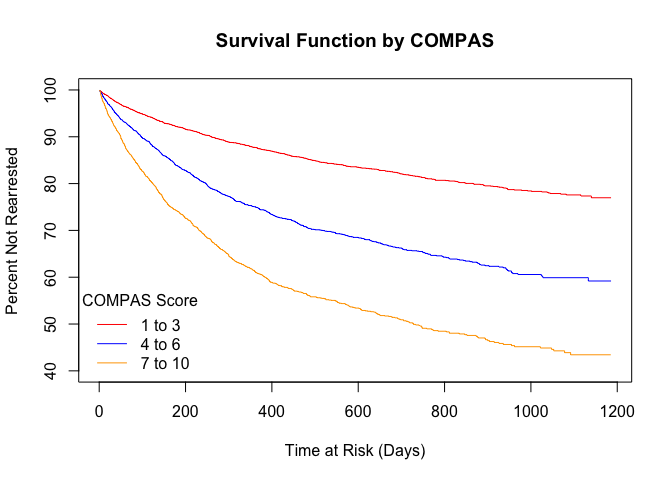
\includegraphics{survival_files/figure-latex/km_curve-2.pdf}

\begin{Shaded}
\begin{Highlighting}[]
\FunctionTok{survdiff}\NormalTok{(survobj}\SpecialCharTok{\textasciitilde{}}\NormalTok{race, }\AttributeTok{data=}\NormalTok{ph)}
\end{Highlighting}
\end{Shaded}

\begin{verbatim}
## Call:
## survdiff(formula = survobj ~ race, data = ph)
## 
##                          N Observed Expected (O-E)^2/E (O-E)^2/V
## race=African-American 5147     1607  1293.97    75.725   142.951
## race=Asian              51        8    16.22     4.167     4.195
## race=Caucasian        3569      814   994.40    32.727    51.230
## race=Hispanic          944      206   275.38    17.480    19.438
## race=Native American    32        6     8.26     0.618     0.621
## race=Other             571      118   170.77    16.305    17.397
## 
##  Chisq= 147  on 5 degrees of freedom, p= <2e-16
\end{verbatim}

\begin{Shaded}
\begin{Highlighting}[]
\NormalTok{ph}\SpecialCharTok{$}\NormalTok{compas }\OtherTok{\textless{}{-}} \FunctionTok{cut}\NormalTok{(ph}\SpecialCharTok{$}\NormalTok{decile\_score, }\AttributeTok{breaks=}\FunctionTok{c}\NormalTok{(}\DecValTok{0}\NormalTok{,}\DecValTok{3}\NormalTok{,}\DecValTok{6}\NormalTok{,}\DecValTok{10}\NormalTok{))}
\NormalTok{fitc }\OtherTok{\textless{}{-}} \FunctionTok{survfit}\NormalTok{(survobj}\SpecialCharTok{\textasciitilde{}}\NormalTok{compas, }\AttributeTok{data=}\NormalTok{ph)}
\FunctionTok{plot}\NormalTok{(fitc, }\AttributeTok{xlab=}\StringTok{"Time at risk of recidivism in Days"}\NormalTok{, }
   \AttributeTok{ylab=}\StringTok{"\% not rearrested"}\NormalTok{, }\AttributeTok{yscale=}\DecValTok{100}\NormalTok{,}
   \AttributeTok{main=}\StringTok{"Survival Distribution by COMPAS"}\NormalTok{,}
   \AttributeTok{col =} \FunctionTok{c}\NormalTok{(}\StringTok{\textquotesingle{}red\textquotesingle{}}\NormalTok{, }\StringTok{\textquotesingle{}blue\textquotesingle{}}\NormalTok{, }\StringTok{\textquotesingle{}orange\textquotesingle{}}\NormalTok{, }\StringTok{\textquotesingle{}yellow\textquotesingle{}}\NormalTok{, }\StringTok{\textquotesingle{}green\textquotesingle{}}\NormalTok{, }\StringTok{\textquotesingle{}purple\textquotesingle{}}\NormalTok{)) }
\FunctionTok{legend}\NormalTok{(}\StringTok{\textquotesingle{}bottomleft\textquotesingle{}}\NormalTok{, }\AttributeTok{legend=}\FunctionTok{levels}\NormalTok{(}\FunctionTok{as.factor}\NormalTok{(ph}\SpecialCharTok{$}\NormalTok{compas)), }\AttributeTok{col =} \FunctionTok{c}\NormalTok{(}\StringTok{\textquotesingle{}red\textquotesingle{}}\NormalTok{, }\StringTok{\textquotesingle{}blue\textquotesingle{}}\NormalTok{, }\StringTok{\textquotesingle{}orange\textquotesingle{}}\NormalTok{, }\StringTok{\textquotesingle{}yellow\textquotesingle{}}\NormalTok{, }\StringTok{\textquotesingle{}green\textquotesingle{}}\NormalTok{, }\StringTok{\textquotesingle{}purple\textquotesingle{}}\NormalTok{), }\AttributeTok{lty=}\DecValTok{1}\NormalTok{)}
\end{Highlighting}
\end{Shaded}

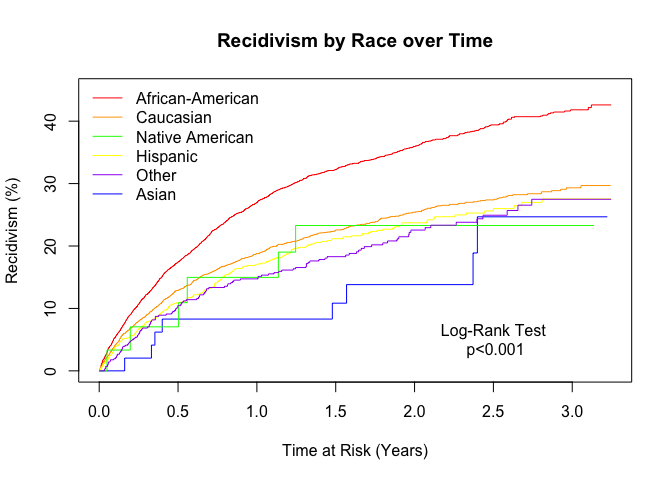
\includegraphics{survival_files/figure-latex/km_curve-3.pdf}

Note: I haven't used this package in a long time so I needed to look how
to use the functions in
\href{https://cran.r-project.org/web/packages/survival/survival.pdf}{documentation}.
As a consultant, you will probably need to read the documentation a lot.

\hypertarget{cox-proportional-hazards-model}{%
\subsection{Cox proportional hazards
model}\label{cox-proportional-hazards-model}}

\begin{itemize}
\item
  Difficult to work with censored data using generalized linear models
\item
  Question: We can use use a GLM here?

  \begin{itemize}
  \tightlist
  \item
    A: Yes
  \item
    B: No
  \item
    C: Not Sure
  \end{itemize}
\item
  Assuming that each individual hazard function is proportional to some
  common baseline hazard function makes the problem workable: \[
  \lambda(t|x_i) = \lambda_0(t) \exp(\beta x_i)
  \] where \(x_i\) is the covariate vector for participant \(i\) and
  \(\beta\) is the parameter vector to be estimated
\item
  \(\lambda_0(t)\) is the hazard function for \(x_i=(0,\dots,0)\)
\item
  \(\exp(\beta x_i)\) explains proportional differences in hazards as
  \(x_i\) changes as in parametric regression
\item
  Then the probability that individual \(j\) experiences an event at
  \(t_{(j)}\) given survival until \(t_{(j)}\) is
  \[\lambda(t_{(j)}|x_{(j)})=\lambda_0(t_{(j)})\exp(x_{(j)}\beta)\]
\item
  The total probability within the sample of an event occurring at time
  \(t_{(j)}\) given those who have survived until \(t_{(j)}\) is
  \[\sum_{k: t_k\geq t_{(j)}} \lambda(t_{(j)}|x_k) = \sum_{k: t_k\geq t_{(j)}} \lambda_0(t_{(j)})\exp(x_k\beta)\]
\item
  Then probability of an event occurring at \(t_{(j)}\) conditioning on
  covariates \(x_{(j)}\) (the likelihood) is \[\begin{align*}
  L_j(\beta) &= P[(j)\text{ fails}|\text{1 failure from those at risk at $t_{(j)}$}]
  = \frac{P[\text{$(j)$ fails}| \text{still at risk}]}{\sum_{k: t_k\geq t_{(j)}}P(\text{$k$ fails}| \text{still at risk})} \\
  &= \frac{\lambda(t_{(j)}|x_{(j)})}{\sum_{k: t_k\geq t_{(j)}} \lambda(t_{(j)}|x_k)} = \frac{\lambda_0(t_{(j)})\exp(x_{(j)}\beta)}{\sum_{k: t_k\geq t_{(j)}} \lambda_0(t_{(j)})\exp(x_k\beta)}
  = \frac{\exp(x_{(j)}\beta)}{\sum_{k: t_k\geq t_{(j)}} \exp(x_k\beta)}
  \end{align*}\]
\item
  Notice that the baseline hazard function, \(\lambda_0(t)\), cancels.
  So, now we can use use an optimization technique to maximize this
  function
\item
  The joint likelihood for the sample is
  \[\tilde L(\beta) = \prod_{j=1}^J L_j(\beta) = \prod_{j=1}^J \frac{\exp(x_{(j)}\beta)}{\sum_{k: t_k\geq t_{(j)}} \exp(x_k\beta)}
  = \prod_{i=1}^n \left[\frac{\exp(x_i\beta)}{\sum_{\ell\in R(t_i)} \exp(x_\ell\beta)}\right]^{\delta_i}\]
\item
  log-likelihood: \[
  \tilde \ell(\beta) = \sum_{j=1}^J\left[ x_{(j)}\beta - \log \left(\sum_{k: t_k\geq t_{(j)}} \exp(x_k\beta) \right)\right]
  \] where \(R(t) = \left\{\ell: t_\ell \geq t\right\}\)
\item
  Maximize the likelihood with Newton-Raphson method
\end{itemize}

\hypertarget{is-compas-racially-biased}{%
\subsubsection{Is COMPAS racially
biased?}\label{is-compas-racially-biased}}

\begin{itemize}
\item
  To determine this, we must use interactions
\item
  Let \(A\) and \(B\) be binary, input variables and \(Y\) a continuous
  outcome

  \begin{itemize}
  \tightlist
  \item
    assume linear regression
  \end{itemize}
\item
  How do we read the output?
\end{itemize}

\begin{longtable}[]{@{}lll@{}}
\toprule
Variable & Coef & p-value \\
\midrule
\endhead
A & 1.5 & 0.01 \\
B & 0.1 & 0.35 \\
A*B & 0.5 & 0.02 \\
\bottomrule
\end{longtable}

\begin{itemize}
\item
  On average, \(Y\) increases by 1.5 when \(A=1\) compared to \(A=0\)
  while controlling for \(B\) and this change is statistically
  significant at an \(\alpha=0.05\) signifiance level
\item
  There is no evidence to suggest that \(B\) is associated with \(Y\)
  (while controlling for \(A\))
\item
  Additionally, \(Y\) increases by 0.5 when both \(A\) and \(B\) are 1
\item
  Changing the baseline race

  \begin{itemize}
  \tightlist
  \item
    R uses alphabetical order so African-American (AA) would be the
    reference group without the \texttt{relevel} command
  \item
    Now, Caucasian (white) is the reference group
  \item
    In most medical literature, white is the reference racial group, but
    this has come under some criticism
  \item
    Here, because AA is of particular interest, we probably don't want
    AA to be the reference group
  \end{itemize}
\item
  We divide age by 10 so that we can interpret change in risk per 10
  years of age
\end{itemize}

\begin{Shaded}
\begin{Highlighting}[]
\NormalTok{ph}\SpecialCharTok{$}\NormalTok{race }\OtherTok{=} \FunctionTok{relevel}\NormalTok{(}\FunctionTok{as.factor}\NormalTok{(ph}\SpecialCharTok{$}\NormalTok{race), }\AttributeTok{ref=}\StringTok{"Caucasian"}\NormalTok{)}
\NormalTok{ph}\SpecialCharTok{$}\NormalTok{age10 }\OtherTok{=}\NormalTok{ ph}\SpecialCharTok{$}\NormalTok{age}\SpecialCharTok{/}\DecValTok{10}
\FunctionTok{summary}\NormalTok{(}\FunctionTok{coxph}\NormalTok{(survobj}\SpecialCharTok{\textasciitilde{}}\NormalTok{race}\SpecialCharTok{*}\NormalTok{decile\_score}\SpecialCharTok{+}\NormalTok{age10, }\AttributeTok{data=}\NormalTok{ph))}
\end{Highlighting}
\end{Shaded}

\begin{verbatim}
## Call:
## coxph(formula = survobj ~ race * decile_score + age10, data = ph)
## 
##   n= 10314, number of events= 2759 
## 
##                                       coef exp(coef) se(coef)      z Pr(>|z|)
## raceAfrican-American               0.25736   1.29351  0.09147  2.814   0.0049
## raceAsian                         -1.81253   0.16324  0.83302 -2.176   0.0296
## raceHispanic                       0.07436   1.07719  0.14092  0.528   0.5977
## raceNative American               -2.44849   0.08642  1.52191 -1.609   0.1077
## raceOther                         -0.21598   0.80575  0.17696 -1.220   0.2223
## decile_score                       0.18448   1.20260  0.01306 14.129  < 2e-16
## age10                             -0.09567   0.90877  0.01875 -5.102 3.36e-07
## raceAfrican-American:decile_score -0.02812   0.97227  0.01560 -1.802   0.0715
## raceAsian:decile_score             0.31320   1.36779  0.12583  2.489   0.0128
## raceHispanic:decile_score         -0.03159   0.96890  0.02780 -1.137   0.2557
## raceNative American:decile_score   0.28200   1.32578  0.17978  1.569   0.1167
## raceOther:decile_score             0.04658   1.04768  0.03587  1.299   0.1941
##                                      
## raceAfrican-American              ** 
## raceAsian                         *  
## raceHispanic                         
## raceNative American                  
## raceOther                            
## decile_score                      ***
## age10                             ***
## raceAfrican-American:decile_score .  
## raceAsian:decile_score            *  
## raceHispanic:decile_score            
## raceNative American:decile_score     
## raceOther:decile_score               
## ---
## Signif. codes:  0 '***' 0.001 '**' 0.01 '*' 0.05 '.' 0.1 ' ' 1
## 
##                                   exp(coef) exp(-coef) lower .95 upper .95
## raceAfrican-American                1.29351     0.7731  1.081223    1.5475
## raceAsian                           0.16324     6.1259  0.031898    0.8354
## raceHispanic                        1.07719     0.9283  0.817225    1.4199
## raceNative American                 0.08642    11.5708  0.004377    1.7064
## raceOther                           0.80575     1.2411  0.569597    1.1398
## decile_score                        1.20260     0.8315  1.172211    1.2338
## age10                               0.90877     1.1004  0.875973    0.9428
## raceAfrican-American:decile_score   0.97227     1.0285  0.942989    1.0025
## raceAsian:decile_score              1.36779     0.7311  1.068836    1.7504
## raceHispanic:decile_score           0.96890     1.0321  0.917530    1.0232
## raceNative American:decile_score    1.32578     0.7543  0.932054    1.8858
## raceOther:decile_score              1.04768     0.9545  0.976552    1.1240
## 
## Concordance= 0.661  (se = 0.005 )
## Likelihood ratio test= 866.1  on 12 df,   p=<2e-16
## Wald test            = 841.2  on 12 df,   p=<2e-16
## Score (logrank) test = 906.8  on 12 df,   p=<2e-16
\end{verbatim}

\begin{itemize}
\item
  Question: Does this model indicate that COMPAS is racially biased?

  \begin{itemize}
  \tightlist
  \item
    A: Yes
  \item
    B: No
  \item
    C: Not Sure
  \end{itemize}
\item
  An interpretation: Compared to Caucasians, a unit increase in the
  COMPAS decile score for African-Americans corresponds to a decrease in
  risk of recidivism by a factor of 0.97; this figure is borderline
  significant (p=0.0715). Said differently, among African-Americans and
  Caucasians with similar COMPAS scores, African-Americans, on average,
  have a 3\% lower risk of recidivism compared to Caucasians. This
  indicates that COMPAS may be assigning higher scores to
  African-American than to Caucasians with a similar risk of recidivism.
  Asians, on the other hand, were assigned lower scores than Caucasians
  with a similar risk of recidivism (p=0.0128). There were no
  differences between other racial groups and Caucasians.
\item
  How can we interpret this model?
\item
  Testing proportional hazards assumption
\item
  Null Hypothesis: Proportional hazards
\item
  Should consider transformation (next lecture)
\end{itemize}

\begin{Shaded}
\begin{Highlighting}[]
\NormalTok{test.ph }\OtherTok{\textless{}{-}} \FunctionTok{cox.zph}\NormalTok{(}\FunctionTok{coxph}\NormalTok{(survobj}\SpecialCharTok{\textasciitilde{}}\NormalTok{race}\SpecialCharTok{+}\NormalTok{age}\SpecialCharTok{+}\NormalTok{decile\_score, }\AttributeTok{data=}\NormalTok{ph))}
\NormalTok{test.ph}
\end{Highlighting}
\end{Shaded}

\begin{verbatim}
##              chisq df      p
## race          6.79  5 0.2367
## age           4.66  1 0.0308
## decile_score  2.98  1 0.0841
## GLOBAL       18.89  7 0.0085
\end{verbatim}

\begin{itemize}
\tightlist
\item
  Using our knowledge of regression with causation (Bayesian Networks
  above), how can we determine if the COMPAS algorithm is racially
  biased?
\end{itemize}

\textbf{Time-Dependent Covariates}

\begin{itemize}
\tightlist
\item
  In cases, covariates can change over time

  \begin{itemize}
  \tightlist
  \item
    Here, zip code, or age can change over time
  \item
    This change may have an effect on the hazard function
  \end{itemize}
\item
  Recall that \(\lambda(t)\) is the instantaneous probability of an
  event at time \(t\) given survival up to \(t\)
\item
  If one or more covariates change over time, \(x(t)\), we can model
  hazard as \[\lambda(t|x(t)) = \lambda_0(t)\exp(\beta x(t))\]
\item
  The partial likelihood become
  \[\tilde L(\beta) = \prod_{i=1}^n \left[\frac{\exp(x_i(t_i)\beta)}{\sum_{\ell\in R(t_i)} \exp(x_\ell(t_i)\beta)}\right]^{\delta_i}\]
\end{itemize}

\textbf{Stratified Models}

\begin{itemize}
\tightlist
\item
  If a sample of \(n\) observations are thought to have \(S\) mutually
  exclusive baseline hazards, we can choose to use a stratified model
  \[\lambda_h(t|x) = \lambda_{0h}(t)\exp(x\beta) \text{ for } h=1,\dots,S\]
\item
  Example: Want to assess effect of age and weight only on risk of
  death, we may want to stratify by gender
\item
  If covariates are assumed to be different in different strata, we can
  estimate strata-specific parameters, \(\beta_h\), for each strata
  \[\lambda_h(t|x) = \lambda_{0h}(t)\exp(x\beta_h) \text{ for } h=1,\dots,S\]
\item
  Partial likelihood:
  \[\tilde L(\beta) = \prod_{h=1}^S \prod_{i=1}^{n_h} \left[\frac{\exp(x_{i(h)}\beta_h)}{\sum_{\ell\in R_h(t_{i(h)})} \exp(x_{\ell(h)\beta_h}))}\right]\]
  where \(n_h\) is the number in each strata, \(i(h)\) is the \(i\)th
  observation in the \(h\)th stratam, \(R_h\) is the stratam specific
  risk set
\end{itemize}

\textbf{Frailty model}

\begin{itemize}
\tightlist
\item
  Some data will have associations among the observations themselves
\item
  Example: COMPAS data could have multiple arrests, their associated
  COMPAS score, and their own follow up
\item
  It is reasonable to assume that past scores, and arrests may provide
  information (association) on future data
\item
  If there are associations among the observations in the data, the
  parameter point estimates will be accurate
\item
  But, standard error will not be correct, so any inference (p-values,
  confidence intervals) will not be valid
\item
  Solution: modify the information sandwich for GLMs with associated
  observations to Cox PH
\item
  This provides a consistent estimator for the covariance matrix
\item
  Note: so far we have not discussed sandwich estimator
\end{itemize}

These notes are based on chapter 9 of Lachin, John M. Biostatistical
methods: the assessment of relative risks. Vol. 509. John Wiley \& Sons,
2009.

\hypertarget{consulting-case-study-treating-syphilis-in-people-living-with-hiv}{%
\subsubsection{Consulting Case Study: Treating Syphilis in People living
with
HIV}\label{consulting-case-study-treating-syphilis-in-people-living-with-hiv}}

\begin{itemize}
\tightlist
\item
  The typically, the first line treatment for syphilis is penicillin
\item
  But, people living with HIV are sometimes thought to be
  immunocompromised
\item
  Because of this, it was common for physicians to administer two or
  more standard doses to treat syphilis for someone living with HIV
\item
  US treatment guidelines in the US recommended one standard dose
  regardless of HIV status
\item
  But, there was disagreement in the medical community on this guideline
\item
  This type of disagreement (equipoise) frequently leads to research
\end{itemize}

\textbf{Background:} Treatment guidelines recommend the use of a single
dose of benzathine penicillin G (BPG) for treating early syphilis in
human immunodeficiency virus (HIV)-infected persons. However, data
supporting this rec- ommendation are limited. We examined the efficacy
of single-dose BPG in the US Military HIV Natural History Study.

\textbf{Methods:} Subjects were included if they met serologic criteria
for syphilis (ie, a positive nontreponemal test {[}NTr{]} confirmed by
treponemal testing). Response to treatment was assessed at 13 months and
was defined by a ≥4-fold decline in NTr titer. Multivariate Cox
proportional hazard regression models were utilized to examine factors
associated with treatment response.

\textbf{Results:} Three hundred fifty subjects (99\% male) contributed
478 cases. Three hundred ninety-three cases were treated exclusively
with BPG (141 with 1 dose of BPG). Treatment response was the same among
those receiving 1 or \textgreater1 dose of BPG (92\%). In a multivariate
analysis, older age (hazard ratio {[}HR{]}, 0.82 per 10-year increase;
95\% con- fidence interval {[}CI{]}, .73--.93) was associated with
delayed response to treatment. Higher pretreatment titers (refer- ence
NTr titer \textless1:64; HR, 1.94 {[}95\% CI, 1.58--2.39{]}) and CD4
counts (HR, 1.07 for every 100-cell increase {[}95\% CI, 1.01--1.12{]})
were associated with a faster response to treatment. Response was not
affected by the number of BPG doses received (reference, 1 dose of BPG;
HR, 1.11 {[}95\% CI, .89--1.4{]}).

\textbf{Conclusion:} In this cohort, additional BPG doses did not affect
treatment response. Our data support the current recommendations for the
use of a single dose of BPG to treat HIV-infected persons with early
syphilis.

\href{https://academic.oup.com/cid/article/60/4/653/2895840}{Ganesan,
Anuradha, Octavio Mesner, Jason F. Okulicz, Thomas O'Bryan, Robert G.
Deiss, Tahaniyat Lalani, Timothy J. Whitman, Amy C. Weintrob, Grace
Macalino, and Brian K. Agan. ``A single dose of benzathine penicillin G
is as effective as multiple doses of benzathine penicillin G for the
treatment of HIV-infected persons with early syphilis.'' Clinical
Infectious Diseases 60, no. 4 (2015): 653-660.}

Look for in paper:

\begin{itemize}
\tightlist
\item
  Data inclusion criteria
\item
  Baseline table for individuals
\item
  Syphilis episodes table
\item
  KM curves
\item
  Cox PH Model
\end{itemize}

\href{http://citeseerx.ist.psu.edu/viewdoc/download?doi=10.1.1.864.7969\&rep=rep1\&type=pdf}{Response
Letter}

\begin{itemize}
\tightlist
\item
  Because of the disagreement, some clinicians wrote a negative response
  to our study
\item
  The response focused mainly on the methods
\end{itemize}

\href{https://academic.oup.com/cid/article/60/9/1444/404706}{Our
Response}

\hypertarget{high-level-summary}{%
\subsection{High Level Summary}\label{high-level-summary}}

\begin{itemize}
\tightlist
\item
  Always explore the data before running regressions and other
  statistical tests. Look at the raw data itself, try to understand
  variable names, variable distributions, missing data, etc
\item
  Survival analysis tools, such as Kaplan-Meier curves and Cox PH
  regression, are helpful when follow times leading up to an event vary
  by observation, especially when censoring occurs.
\item
  It is important to be aware of possible causal pathways. But, most of
  the time, it is not possible to use statistical models alone to
  attribute a causal relationships.
\end{itemize}

\end{document}
